\chapter{Algoritmus triangulácie regulárnej implicitne definovanej plochy}
\label{kap:algoritmus}
Po preskúmaní triangulačných algoritmov sme sa v našej práci rozhodli venovať čo najkvalitnejšiemu
prevedeniu triangulácie s menším dôrazom na rýchlosť výpočtu. Ako základnú štruktúru sme použili 
postup, ktorí uviedli autori článku \cite{hilton1996marching}. Tento algoritmus využíva 
\textit{Delaunayovu podmienku} predstavenú v kapitole \ref{kap:delaunay_triangulation}.
Daný algoritmus je implementovaný ako prechod cez frontu, v ktorej sa na úvod nachádzajú
hrany počiatočného trojuholníka, v každom kroku vyberieme z fronty jednu hranu $E$ a pre túto
hranu vykonáme nasledujúcu postupnosť krokov:
\begin{enumerate}
    \item{Vytvoríme vrchol $x_{proj}$ tak, ako sme opísali v kapitole \ref{kap:marching_triangles}, teda 
    ako bod ležiaci v kolmej vzdialenosti $k$ od stredu hrany $E = (x_i, x_j)$ 
    v rovine susedného trojuholníka $T$.}
    \item{Nájdeme vrchol $x_{new}$ ako vrchol, ktorý leží na povrchu a je blízko k bodu 
    $x_{proj}$. Tento bod premietame na plochu v smere $\nabla F(x_{proj})$.
    Platí teda, že $F(x_{new}) = 0$.}
    \item{Skončíme ak je splnená jedna z nasledujúcich možností:
    \begin{itemize}
        \item{Vrchol $x_{new}$ leží na hranici, teda medzi hraničnými 
        hranami sa nachádza hrana s vrcholom $x_{new}$.}
        \item{Normála $\vec{n}_{new}$ trojuholníka $T_{new}$ ktorého vrcholy sú $x_i, 
        x_j, x_{new}$ je opačná ako
        normála $\vec{n}$ susedného trojuholníka $T$, teda 
        $\vec{n}_{new} \cdot \vec{n} < 0$.}
    \end{itemize}
    }
    \item{Nech $B_{new}$ je \textit{Delaunayova guľa} trojuholníka $T_{new}$.
        Pre trojuholník $T_{new}$ overíme platnosť \textit{Delaunayovej podmienky}, 
    ktorú sme predstavili v kapitole \ref{kap:delaunay_triangulation}, ak podmienka platí
    vykonáme nasledujúce kroky a prejdeme na ďalšiu hranu.
    \begin{itemize}
        \item{Pridáme vrchol $x_{new}$ do zoznamu vrcholov.}
        \item{Pridáme trojuholník $T_{new}$ do meshu.}
        \item{Pridáme hrany $(x_i, x_{new})$ a 
        $(x_j, x_{new})$ do fronty s hranami.}
    \end{itemize}
    }
    \item{
        Ak \textit{Delaunayova podmienka} z bodu $4$ neplatí overíme platnosť \textit{Delaunayovej podmienky} 
        pre trojuholníky 
        $T_{prev} = \bigtriangleup(x_i, x_j, x_{prev})$ a 
        $T_{next} = \bigtriangleup(x_i, x_j, x_{next})$, kde 
        $x_{prev}$ a $x_{next}$ sú hraničné vrcholy,
        pričom $x_{prev}$ 
        je sused vrchola $x_i$ a $x_{next}$ je sused vrchola 
        $x_j$. Ak niektorý z nich podmienku
        spĺňa, vykonáme preň body z kroku 4 a prejdeme na ďalšiu hranu.
    }
    \item{
        Ak trojuholníky $T_{new}$, $T_{prev}$ ani $T_{next}$ nespĺňajú podmienku, potom 
        ak \textit{Delaunayova guľa} obsahuje hraničný vrchol $x_{overlap} \in B_{new}$ nejakého hraničného 
        trojuholníka $T_{overlap}$. Trojuholník $T_{overlap}$ je rovnako orientovaný ako hraničný 
        trojuholník $T$, teda platí $\vec{n} \cdot \vec{n}_{overlap} > 0$. 
        Overíme platnosť \textit{Delaunayovej podmienky} pre 
        trojuholník $T_{overlap}$, kde $x_{overlap}$ je najbližší k hrane $E$ zo všetkých hraničných
        vrcholov, ktoré sa nachádzajú v Delaunayovej guli. Ak podmienku spĺňa aplikujeme naň body z 
        kroku 4 a prejdeme na ďalšiu hranu.
    }
    \item{
        Ak žiadny trojuholník nebol pridaný do meshu, testovanie hrany $E$ skončíme.
    }
\end{enumerate}

Tento algoritmus používame v našej práci ako základnú štruktúru a pridávame do neho ďalšie podmienky 
a postupy na skvalitnenie výslednej triangulácie. 

\section {Štruktúra algoritmu}
\label{kap:first_part_of_algorithm}

Náš algoritmus sleduje plochu.
Funguje na princípe postupného pridávania trojuholníkov do rozpracovaného meshu. V každom kroku
pridávame najviac jeden trojuholník.

\subsection{Vstupné dáta}
\label{kap:input_data}
Cieľom práce je skonštruovať a naprogramovať algoritmus, ktorý vytrianguluje ľubovoľnú hladkú plochu s 
možnosťou zadania presnosti triangulácie. Na vstupe algoritmu sú preto nasledujúce dáta:
\begin{itemize}
    \item{
        Funkcia $F$ zadaná implicitne.
        
        Nech $F:\mathbb{R}^3 \to \mathbb{R}$.
        Nulová hladina tejto funkcie, t.j. $\{x \in \mathbb{R}^3 : F(x) = 0\} = S$ určuje plochu, 
        ktorú chceme triangulovať. 
        Zadaná plocha musí byť bez singularít, t.j. $\nabla F(x) \neq 0 \,\, \forall x \in S.$
    }
    \item{
        Veľkosť hrany $a$ trojuholníka.

        Toto je približná veľkosť hrany trojuholníka v triangulácii. 
        Čím je veľkosť hrany menšia, tým je triangulácia presnejšia. Veľkosť hrany trojuholníka 
        nesmie byť však príliš veľká. Malá veľkosť hrany zvyčajne nevadí, avšak pre 
        menšie trojuholníky trvá algoritmus omnoho dlhšie. Na obrázku \ref{obr:time_edge_size}
        vidíme graf závislosti času od dĺžky hrany pre jednotkovú sféru pre náš algoritmus. 
        Tento algoritmus môžeme
        naprogramovať aj omnoho efektívnejšie, my sme však algoritmus na čas neoptimalizovali.

        \begin{figure}
            \centerline{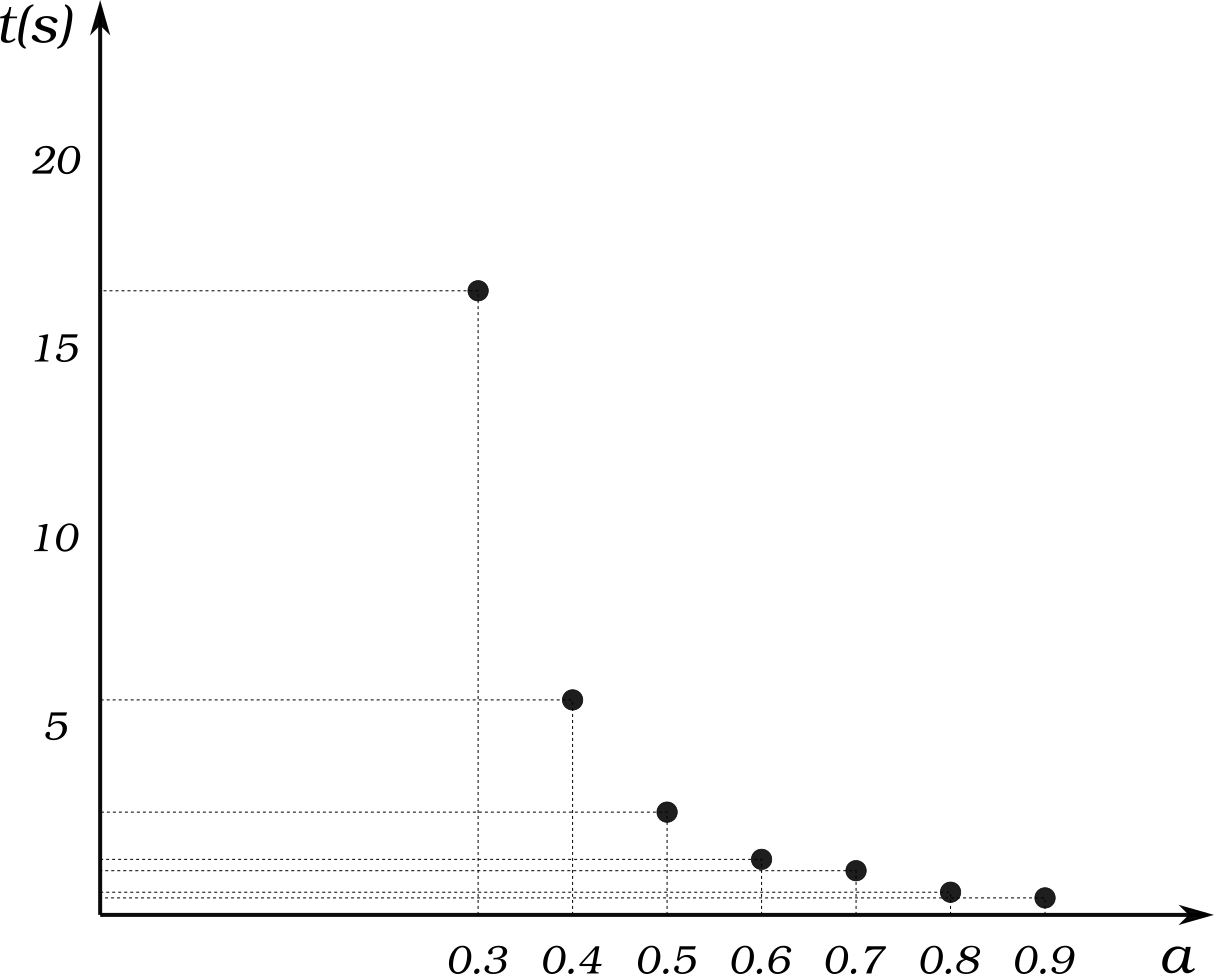
\includegraphics[width=0.45\textwidth]{images/time_edge_size}}
            \caption[Graf závislosti času od veľkosti hrany]{Graf závislosti času od veľkosti hrany pre jednotkovú sféru.}
            %id obrazku, pomocou ktoreho sa budeme na obrazok odvolavat
            \label{obr:time_edge_size}
        \end{figure}
    }
    \item{
        Počiatočný bod $x_{seed}$, v ktorom začneme trianguláciu povrchu. 

        Tento bod musí ležať na povrchu alebo dostatočne blízko na povrchu.
    }
    \item{
        Ohraničenie.

        Pre ohraničenú trianguláciu potrebujeme zadať hranicu ohraničenia. Pre každú z troch súradníc 
        sú to 2 čísla, minimum a maximum, teda spolu 6 čísel.
    }
\end{itemize}

Začneme vytvorením jediného trojuholníka s veľkosťou hrany približne $a$, presný spôsob implementácie
opíšeme v kapitole \ref{kap:implementation}.

Funkčnosť algoritmu opíšeme indukčne. Majme korektnú čiastočnú trianguláciu povrchu, na začiatku
je to jediný trojuholník. Prvá otázka, ktorú si kladieme, je nasledujúca. 
\textit{Aké podmienky musí spĺňať trojica vrcholov} $x_i, x_j, x_k$ 
\textit{aby sme ju pridali do triangulácie ako nový trojuholník na hraničnej hrane} $E = (x_i, x_j)?$ 

\subsection{Pridanie trojuholníka do meshu}
\label{kap:triangle_conditions}

Majme hraničnú hranu $E=(x_i, x_j)$ čiastočnej triangulácie $M$ a bod $x_k \in \mathbb{E}^3$. 
Tento bod sa môže aj nemusí nachádzať medzi vrcholmi $M$. Za akých podmienok môžeme pridať trojuholník 
$T=(x_i, x_j, x_k)$ do $M$?

\begin{enumerate}
    \item{
        \textit{Trojica bodov tvorí trojuholník.}


        Veľmi zjavná avšak veľmi dôležitá podmienka. Ak by sme však overovali klasickú 
        \textit{trojuholníkovú nerovnosť} vyradili by sme iba kolineárne trojice bodov. My však nechceme 
        umožniť ani tvorbu extrémne úzkych trojuholníkov, preto upravíme podmienku aby vyradila aj tieto
        trojuholníky a to tak, že súčet dĺžok každej dvojice strán musí byť väčší od dĺžky tretej aspoň
        o nejakú malú konštantu $z$. Túto konštantu je vhodné voliť napríklad na základe zadanej dĺžky 
        hrany trojuholníka $a$. V našom algoritme používame konštantu $z = 0.01 a$. 
    } 

    \item{
        \textit{Trojuholník je správne orientovaný.}


        Čo znamená správna orientácia môžeme vidieť na obrázku \ref{obr:good_orientation}. Uhol $\beta$
        počítame ako orientovaný uhol dvoch vektorov $\overrightarrow{x_i x_j}$ a $\overrightarrow{x_i x_{new}}$.
        Zaujíma nie len veľkosť uhla ale aj orientácia vzhľadom na susedný trojuholník. To 
        vyjadríme znamienkom pri veľkosti uhla. 

        \begin{figure}
            \centerline{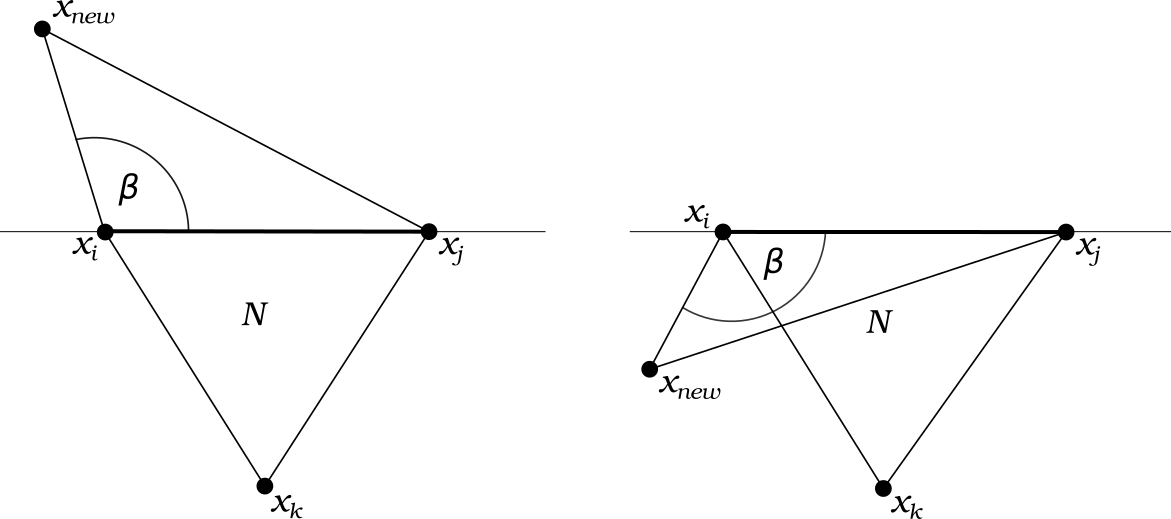
\includegraphics[width=0.55\textwidth]{images/good_orientation}}
            \caption[Orientácia bázy vzhľadom na referenčnú bázu]
            {$T(x_i, x_j, x_{new})$ \textit{naľavo} má opačnú orientáciu ako referenčná báza, 
            trojuholník \textit{napravo} má rovnakú orientáciu.}
            %id obrazku, pomocou ktoreho sa budeme na obrazok odvolavat
            \label{obr:good_orientation}
        \end{figure}

        Pod orientáciou vzhľadom na susedný trojuholník myslíme nasledovné.
        Ak

        \begin{equation}
        \label{eq:vector_space_orientation}
        (\overrightarrow{x_i x_j} \times \overrightarrow{x_i x_k}) 
        \cdot (\overrightarrow{x_i x_j} \times \overrightarrow{x_i x_{new}}) < 0
        \end{equation}

        tak je uhol vektorov $\overrightarrow{x_i x_j}$ a $\overrightarrow{x_i x_{new}}$ v intervale $(0, \pi)$, inak 
        je uhol v intervale $ \langle -\pi, 0 \rangle$.
        
        Význam vzťahu \ref{eq:vector_space_orientation} spočíva v koncepte orientácie vektorového 
        priestoru. 

        Zvoľme ako referenčnú bázu priestoru $\mathbb{R}^3$ bázu $(b_0, b_1, b_2)$, takú, že
        $$b_0 = \overrightarrow{x_i x_j},$$
        $$b_1 = \overrightarrow{x_i x_k},$$
        $$b_2 = \overrightarrow{x_i x_j} \times \overrightarrow{x_i x_k}.$$

        Potom trojuholník $T(x_i, x_j, x_{new})$ je \textit{správne} orientovaný, ak je súradnicová 
        sústava $(\overrightarrow{x_i x_j}, \overrightarrow{x_i x_{new}}, \overrightarrow{x_i x_j} \times \overrightarrow{x_i x_{new}})$
        orientovaná opačne ako referenčná súradnicová sústava. To je práve vtedy, keď platí vzťah 
        \ref{eq:vector_space_orientation}, teda keď je $\beta \in (0, \pi)$.
        V našej implementácii však nechceme príliš úzke trojuholníky, túto podmienku sme teda 
        upravili na podmienku
        $\beta \in (\frac{\pi}{10}, \frac{9\pi}{10})$. Vizualizáciu oblasti, z ktorej sú vhodné 
        vrcholy pre trojuholník $T$ a jeho hraničnú hranu $E$ môžeme vidieť na obrázku 
        \ref{obr:good_orientation_points}.

        \begin{figure}
            \centerline{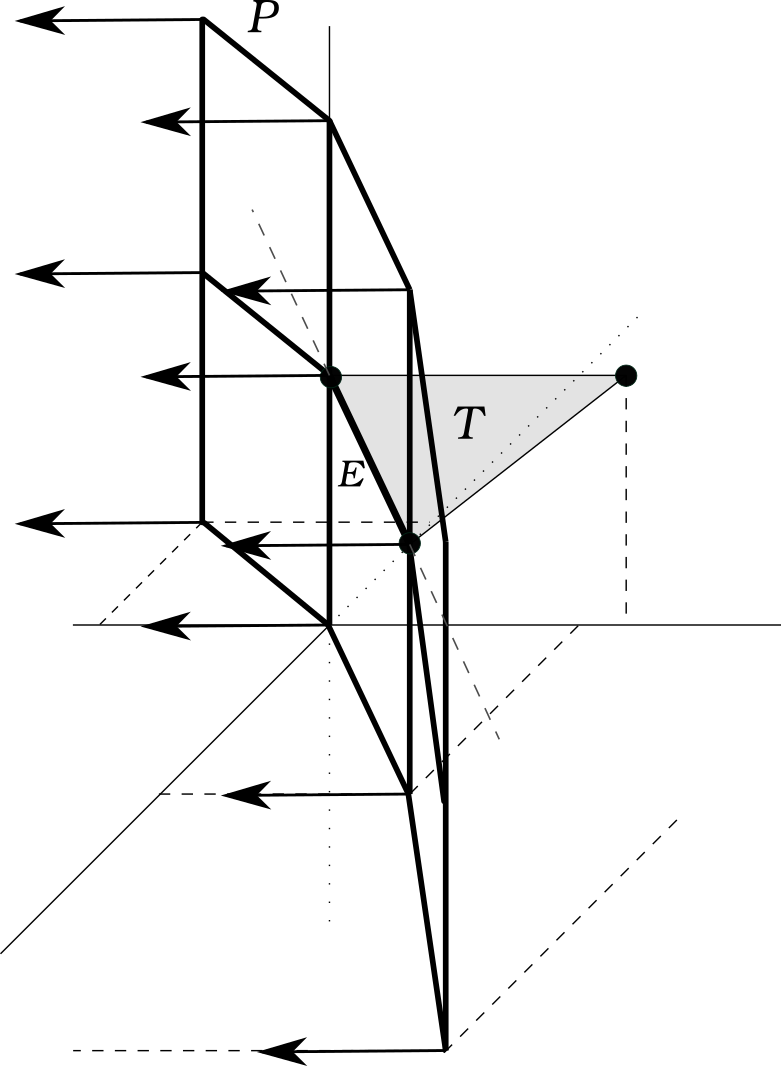
\includegraphics[width=0.25\textwidth]{images/good_orientation_points}}
            \caption[Ilustrácia priestoru vyhovujúcich nových bodov]
            {Vyhovujúce body sa nachádzajú \textit{naľavo} od plochy $P$.}
            %id obrazku, pomocou ktoreho sa budeme na obrazok odvolavat
            \label{obr:good_orientation_points}
        \end{figure}

        Oblasti, v ktorých by sme pri triangulácii potrebovali, aby mali susedné 
        trojuholníky uhol normál väčší ako $\frac{\pi}{2}$, sú oblasti s veľkým zakrivením. 
        V týchto oblastiach musíme buď zmenšiť veľkosť hrany trojuholníka
        pre celý model alebo v adaptívnej verzii v takýchto oblastiach 
        prispôsobiť veľkosť trojuholníkov. 
    }

     \item{
         \textit{Pre nové hrany $(x_i, x_{new})$ a $(x_j, x_{new})$ platí jedna z nasledujúcich podmienok
         \begin{enumerate}
            \item {
                Hrana je \textit{nová}, teda sa nenachádza medzi doterajšími hranami meshu. 
            }
            \item {
                Ak sa hrana nachádza v meshu, tak je \textit{hraničná}.
            }
         \end{enumerate}
         }
     }

     \item{
         \textit{Pre trojuholník je splnená \textit{Delaunayova podmienka} tak, ako bola opísaná v 
         definícii \ref{def:delaunay_constraint}.}

        Ako neskôr uvidíme, túto podmienku nemusia nutne spĺňať všetky trojuholníky. Náš algoritmus sa bude 
        skladať z dvoch častí, v prvej časti vyžadujeme od všetkých trojuholníkov splnenie tejto podmienky.
        Po skončení prvej časti zostávajú v meshi diery, ktoré je možné vyplniť trojuholníkmi nespĺňajúcimi 
        \textit{Delaunayovu podmienku}. Príklad takejto diery môžeme vidieť na obrázku 
        \ref{obr:non_delaunay_triangle}. Hrubšie hrany vyjadrujú hraničné hrany triangulácie. 
        Vidíme, že by sme chceli vytvoriť trojuholník $T = (x_i, x_j, x_k)$,
        avšak tento trojuholník nespĺňa \textit{Delaunayovu podmienku}. Takéto trojuholníky
        budeme riešiť v druhej časti algoritmu.
     }

     \item{
         \textit{V okolí bodu $x_{new}$ sa nenachádza ťažisko už existujúceho trojuholníka.}

         Táto podmienka, tak isto ako \textit{Delaunayova podmienka}, nebude musieť byť splnená vždy,
         avšak taktiež ju vyžadujeme v prvej časti algoritmu. 
         
         Túto podmienku sme zvolili preto, že vo veľkej miere eliminuje problémy s pretínaním 
         trojuholníkov, ak overujeme Delaunayovu podmienky iba pre trojuholník, ktorý chceme pridať,
         avšak nie pre všetky trojuholníky meshu. Tento problém si všimli aj autori S. Akkouche a 
         E. Gallin \cite{akkouche2001adaptive}, ktorí navrhli ako riešenie pri pridávaní trojuholníka 
         overovať \textit{Delaunayovu podmienku} aj pre už existujúce trojuholníky. 
         
         Prístup sme otestovali a myslíme si, že je príliš prísny a zbytočne odmieta aj trojuholníky, 
         ktoré sa nám zdajú vhodné. Navyše vznikajú pomerne rozsiahle diery, ktoré sa nie vždy podarí 
         vhodne opraviť, keďže v časti algoritmu pre opravovanie dier sa už neoveruje
         \textit{Delaunayova podmienka}.

         Ťažisko trojuholníka sme ako oporný bod zvolili z viacerých dôvodov.
         \begin{itemize}
            \item{
                \textit{Je vždy vnútri trojuholníka.}

                Hlavný problém, prečo overovanie Delaunayovej podmienky pre všetky trojuholníky spôsobuje
                odmietanie aj vhodných trojuholníkov je ten, že stred opísanej kružnice nemusí byť vždy
                vnútri trojuholníka. Čím je trojuholník užší, tým je dokonca vzdialenejší a tak môže aj
                vzdialenejší úzky trojuholník spôsobiť nevzniknutie vhodného trojuholníka. 
            }
            \item{
                \textit{Lepšie vystihuje polohu trojuholníka.}

                Ak chceme zabrániť tvorbe prekrývajúcich sa trojuholníkov je pre nás dôležité zaujímať sa 
                o polohu ostatných trojuholníkov v meshi. Ťažisko sa nám zdá ako najvhodnejší bod na 
                vystihnutie tejto polohy.
            }
            \item{
                \textit{Vieme ho jednoducho vypočítať.}

                Mohli by sme počítať aj priamo pretínanie trojuholníkov, to je však v $3D$ pomerne 
                výpočtovo náročný proces, kdežto ťažisko trojuholníka a takisto jeho vzdialenosť od 
                bodu vieme vypočítať veľmi jednoducho.
            }
         \end{itemize}
         
         \begin{figure}
         \centerline{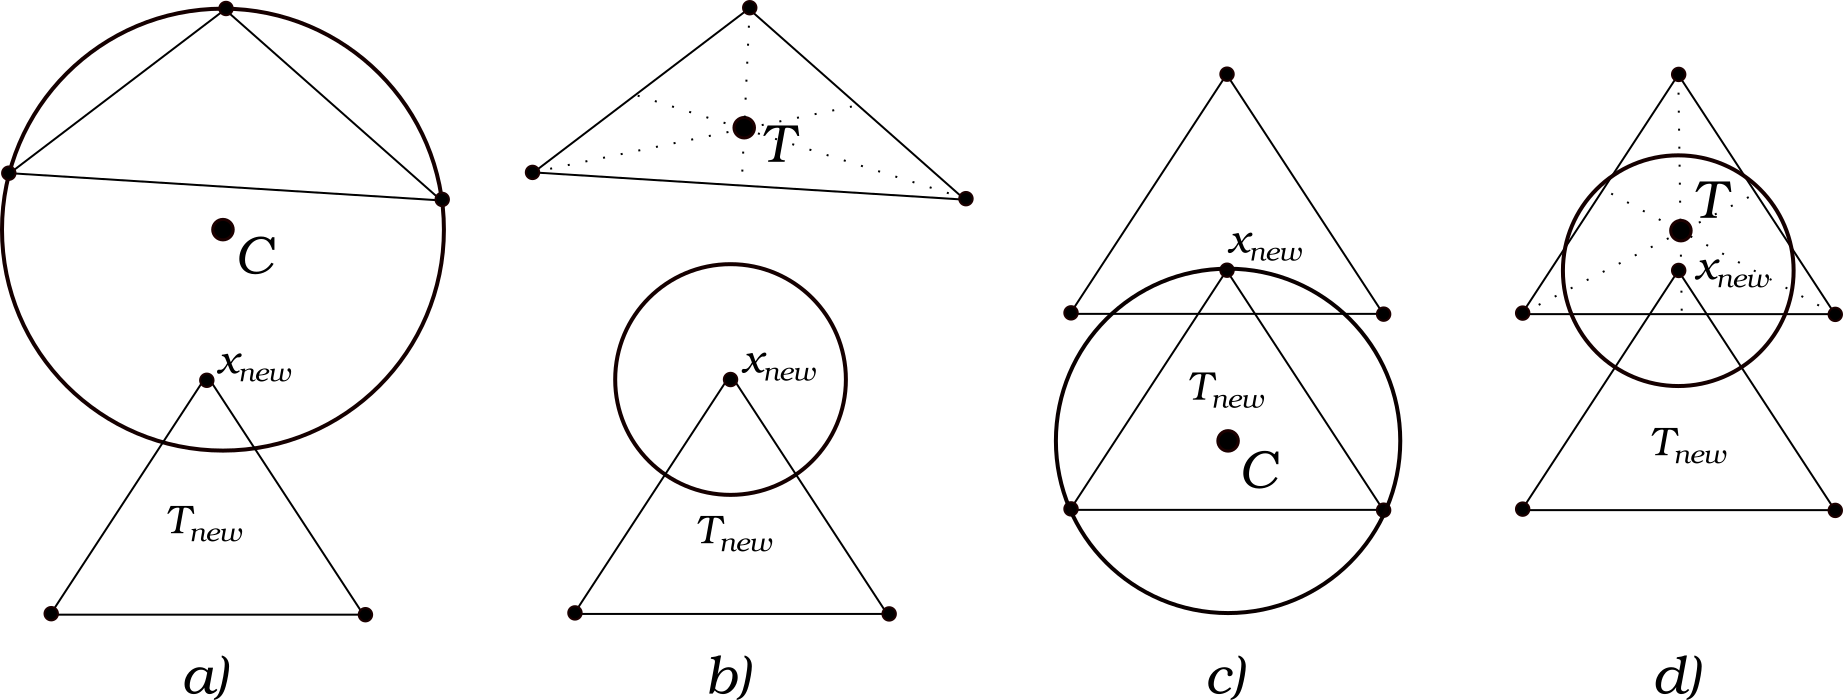
\includegraphics[width=0.8\textwidth]{images/delaunay_vs_gravitycenter_2}}
         \caption[Nová podmienka pre blízkosť ťažiska k novému vrcholu]
         {Vizualizácia novej podmienky pre blízkosť ťažiska k novému vrcholu.}
         %id obrazku, pomocou ktoreho sa budeme na obrazok odvolavat
         \label{obr:delaunay_vs_gravitycenter_2}
         \end{figure}
         
         Na obrázku \ref{obr:delaunay_vs_gravitycenter_2} môžeme vidieť:
         \begin{enumerate}[a)]
            \item{
                Nový vrchol $x_{new}$ nespĺňa Delaunayovu podmienku už existujúceho trojuholníka aj 
                napriek tomu, že trojuholník $T_{new}$ môžeme bez problémov vytvoriť a 
                neporušíme konzistenciu triangulácie.
            }
            \item{
                Nový vrchol $x_{new}$ spĺňa podmienku a môžeme pridať trojuholník $T_{new}$ do meshu.
            }
            \item{
                Trojuholník $T_{new}$ spĺňa \textit{Delaunayovu podmienku} pre trojuholník $T_{new}$ 
                avšak prekrýva sa s už existujúcim trojuholníkom.
            }
            \item{
                Nový vrchol $x_{new}$ sa nachádza v blízkosti ťažiska existujúceho trojuholníka, 
                teda trojuholník $T_{new}$ nespĺňa našu podmienku a do meshu ho nepridáme. 
            }
         \end{enumerate}


         Na obrázku \ref{obr:delaunay_vs_gravitycenter} môžeme vidieť ten 
         istý algoritmus s rovnakými parametrami spustený bez časti, ktorá uzatvára diery. 
         
         Naľavo vidíme výsledok dosiahnutý pri prístupe, ktorý v \textit{Delaunayovej podmienke} overuje aj
         Delaunayovu podmienku ostatných trojuholníkov. 
         
         Napravo vidíme výsledok, ktorý v Delaunayovej
         podmienke overuje blízkosť ťažiska ostatných trojuholníkov. Napriek tomu, že algoritmus
         je v oboch prípadoch spustený bez časti, ktorá uzatvára diery, v druhom prípade je výsledná 
         triangulácia bez dier. Avšak vo veľkej väčšine prípadov podmienka eliminuje problémy, 
         ktoré vznikali pri overovaní \textit{Delaunayovej podmienky} iba pre trojuholník, ktorý pridávame.
     }

    \begin{figure}
        \centerline{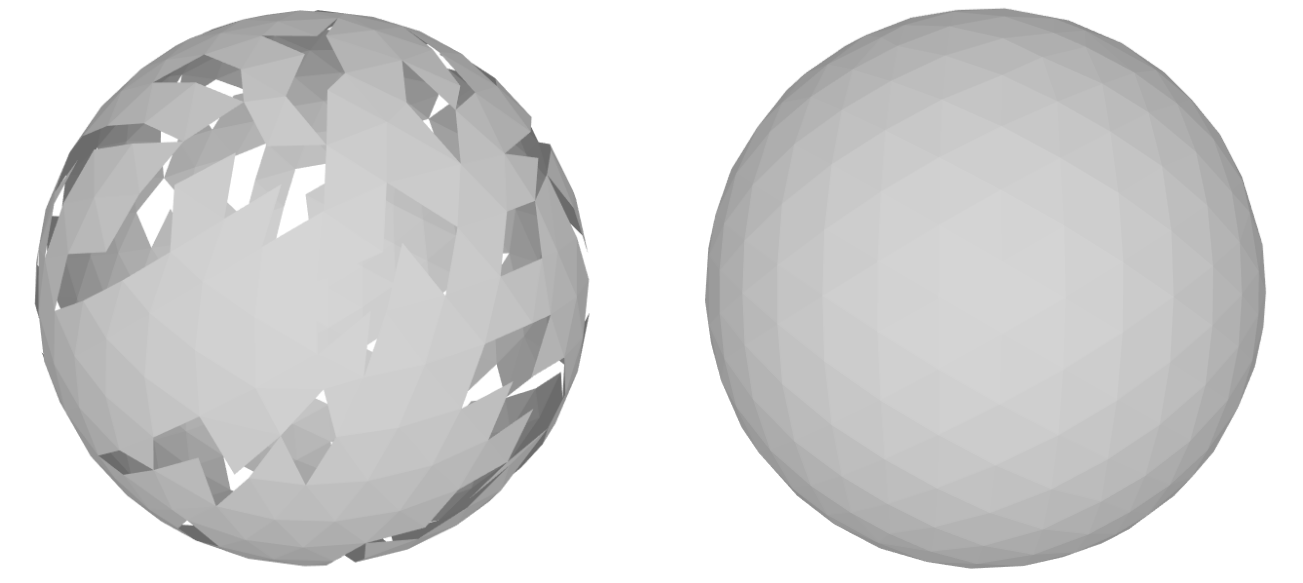
\includegraphics[width=0.75\textwidth]{images/delaunay_vs_gravitycenter}}
        \caption[Delaunayova podmienka verzus podmienka overujúca blízkosť ťažiska]
        {Overovanie \textit{Delaunayovej podmienky} pre všetky trojuholníky(vľavo), overovanie
        podmienky s blízkosťou ťažiska(vpravo).}
        %id obrazku, pomocou ktoreho sa budeme na obrazok odvolavat
        \label{obr:delaunay_vs_gravitycenter}
    \end{figure}

    \begin{figure}
        \centerline{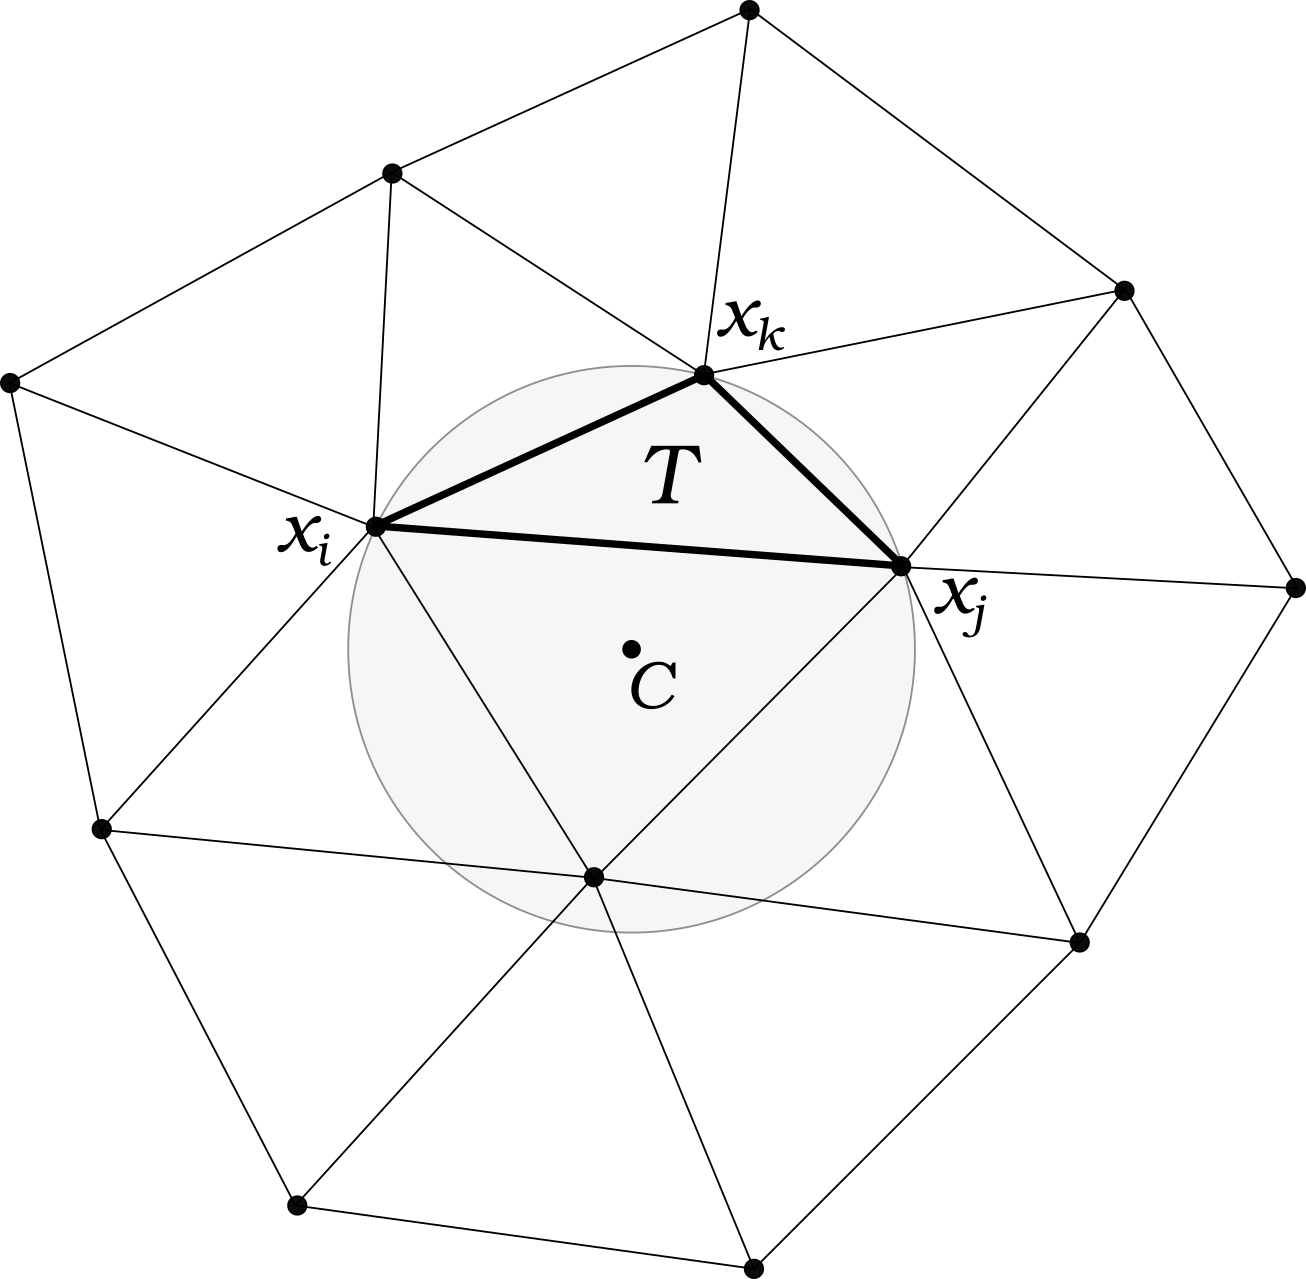
\includegraphics[width=0.35\textwidth]{images/non_delaunay_triangle}}
        \caption[Trojuholník nespĺňajúci \textit{Delaunayovu podmienku}]
        {Vhodný trojuholník nespĺňajúci \textit{Delaunayovu podmienku}.}
        %id obrazku, pomocou ktoreho sa budeme na obrazok odvolavat
        \label{obr:non_delaunay_triangle}
    \end{figure}
\end{enumerate}

Po splnení týchto piatich podmienok pridávame trojuholník do meshu. Avšak ešte potrebujeme zistiť 
ako získať ideálny bod $x_k$.

\subsection{Voľba nového vrchola}
\label{kap:finding_new_vertex}

V každom kroku algoritmu vyberieme zo zoznamu hraničných hrán jednu hranu $E$. Pre túto hranu si 
označíme \textit{susedný trojuholník} ako $N$, tento trojuholník je jediný trojuholník v meshi, 
ktorý má ako jednu z hrán $E$. 

\begin{enumerate}
    \item{
        Vytvoríme bod $x_{proj}$ rovnako, ako v základnom algoritme. Vzdialenosť $k$ volíme
        ako $\frac{\sqrt 3}{2} \, a$, keďže toto je výška rovnostranného trojuholníka so stranou $a$.
    }
    \item{
        Vytvoríme vrchol $x_{new}$ tak, že premietneme bod $x_{proj}$ na plochu $F$ v smere 
        $\vec{v} = \nabla F(x_{proj})$. Ilustráciu postupu vidíme na obrázku \ref{obr:projecting_point}.

        \begin{figure}
            \centerline{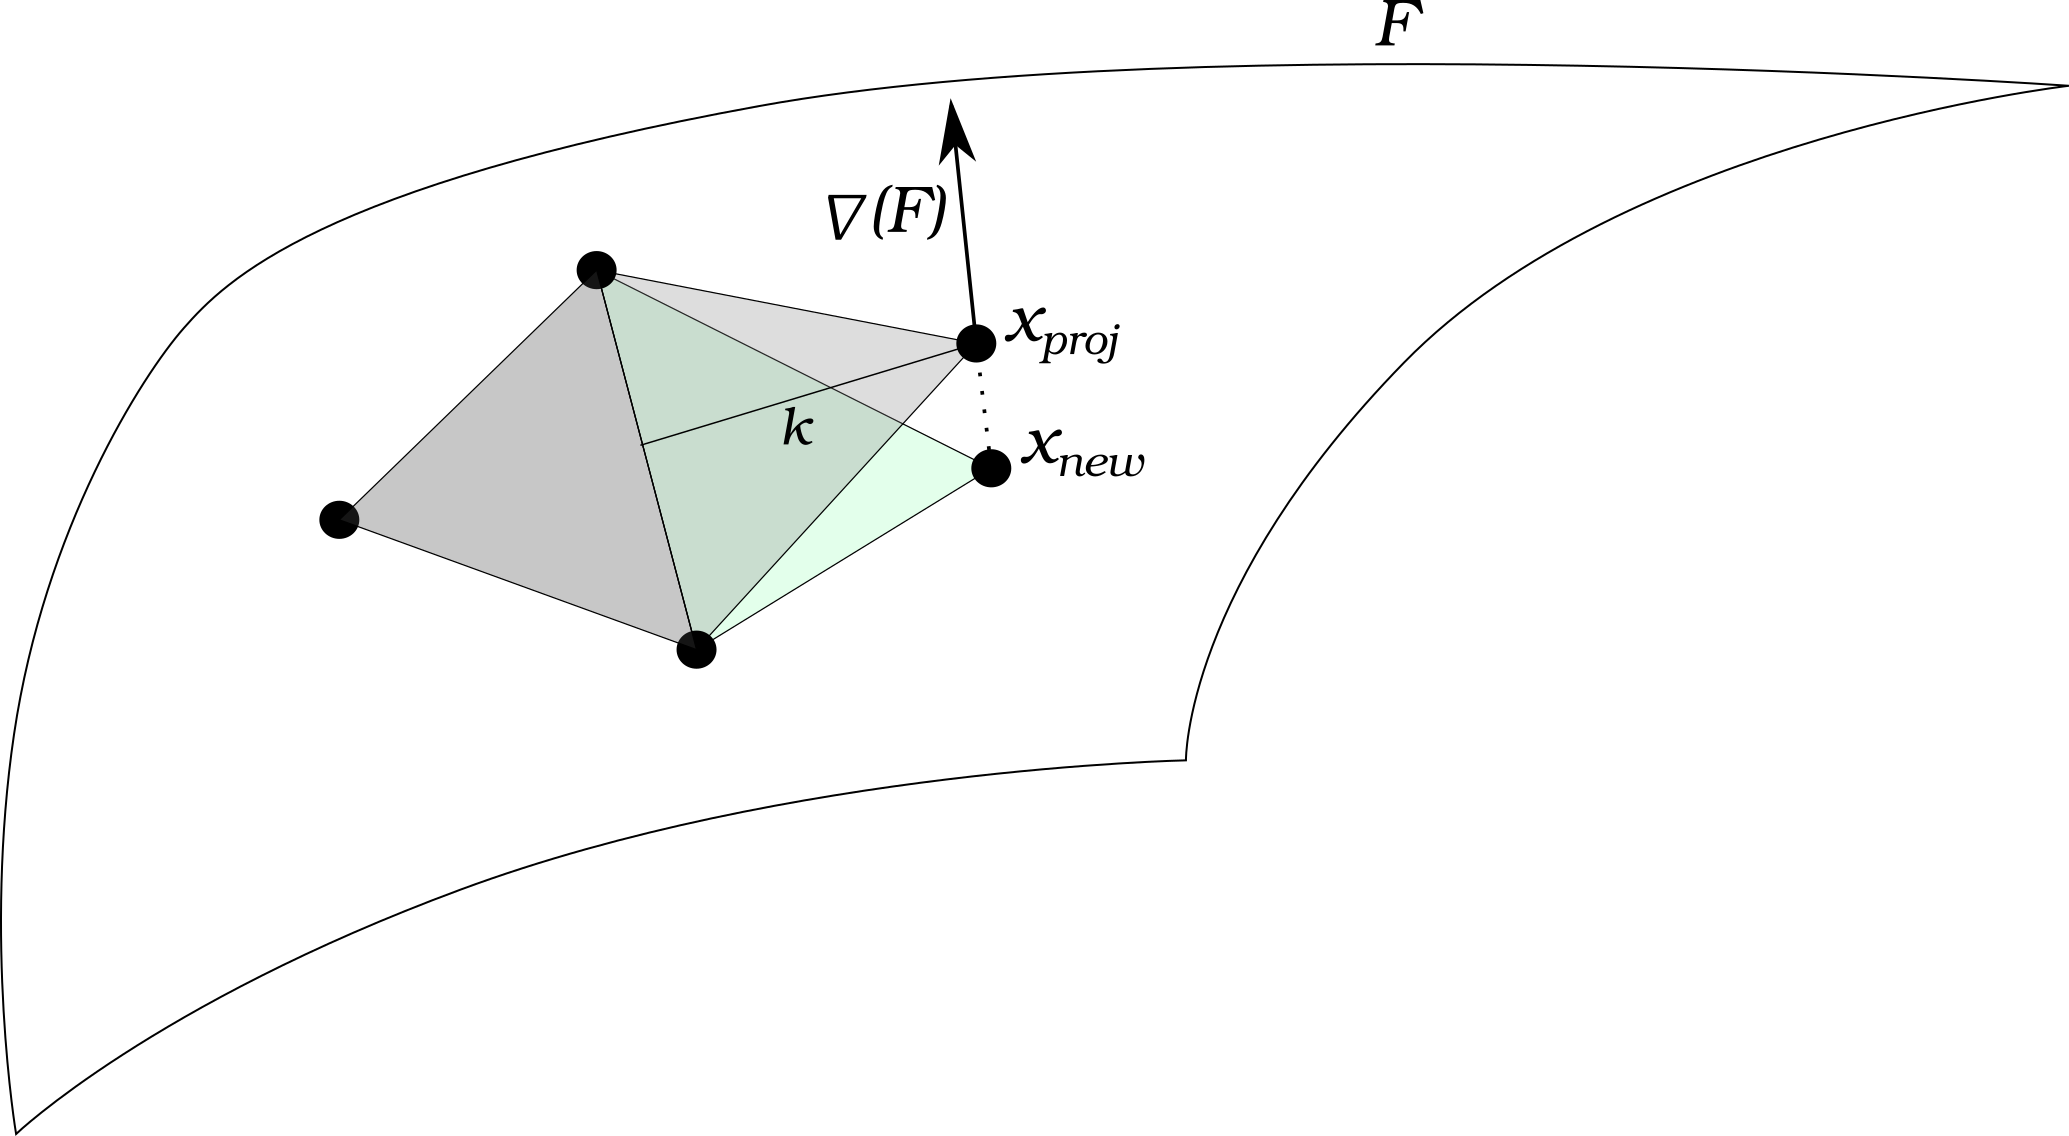
\includegraphics[width=0.5\textwidth]{images/projecting_point}}
            \caption[Premietanie bodu na zadanú plochu]{Premietanie bodu na plochu.}
            %id obrazku, pomocou ktoreho sa budeme na obrazok odvolavat
            \label{obr:projecting_point}
        \end{figure}

        V tomto momente sa z premietania 
        stáva problém hľadania koreňa funkcie $F$ na priamke 
        $\{x_{proj} + t \cdot \nabla F(x_{proj}) | t \in \mathbb{R}\}$.  
        Tu využívame
        \textit{Newtonovu-Raphsonovu metódu} opísanú v kapitole \ref{kap:numeric_methods}. Ako sme 
        už písali, táto metóda je rýchla, ale nie je najspoľahlivejšia. Ak zlyhá,
        použijeme konzervatívnu \textit{metódu bisekcie}.
    }
    \item{
        V prípade, že sa bod $x_{new}$ rovná nejakému hraničnému vrcholu, rovno ho s týmto vrcholom
        spojíme. Táto situácia síce znie ako nepravdepodobná, ale pri útvaroch obsahujúcich rovné plochy sa
        deje pravidelne. Bez tohto kroku sa bod $x_{new}$ nemusí spojiť práve s týmto bodom, ale
        môže vytvoriť trojuholník, ktorý má horší pomer strán.
    }
    \item{
        V prípade, že $x_{prev} = x_{next}$, teda v meshi je diera v tvare trojuholníka, pridáme tento 
        trojuholník do meshu. Tento krok sme pridali, pretože je pomerne častý, jednoduchý a rýchly.
    }
    \item{
        Nájdeme všetky hraničné vrcholy, ktoré sa nachádzajú v \textit{Delaunayovej guli} pre trojuholník 
        $T_{new} = (x_i, x_j, x_{new})$ a usporiadame ich od najbližšieho k hrane $E$. Pri usporiadavaní 
        používame metriku definovanú nasledovne.

        \begin{definition} Vzdialenosť hrany $E=(A,B)$ a vrchola $P$ definujeme ako
        \label{def:segment_point_distance}
        \begin{itemize}
            \item{
                $|AP|$, ak $\measuredangle BAP \in (\frac{\pi}{2}, \frac{3\pi}{2}),$
            }

            \item{
                $|BP|$, ak $\measuredangle ABP \in (\frac{\pi}{2}, \frac{3\pi}{2}),$
            }

            \item{
                $|EP|$ inak.
            }

            
            Pričom $|AP|$, $|BP|$ je euklidovská vzdialenosť bodov v $\mathbb{R}^3$ a $|EP|$ je 
            vzdialenosť bodu $P$ od priamky, na ktorej leží hrana $E$.
        \end{itemize}

        \end{definition}

        Vizualizáciu tejto metriky môžeme vidieť na obrázku \ref{obr:edge_vertex_distance} a izočiary 
        metriky na obrázku \ref{obr:isocurves}.

        \begin{figure}
            \centerline{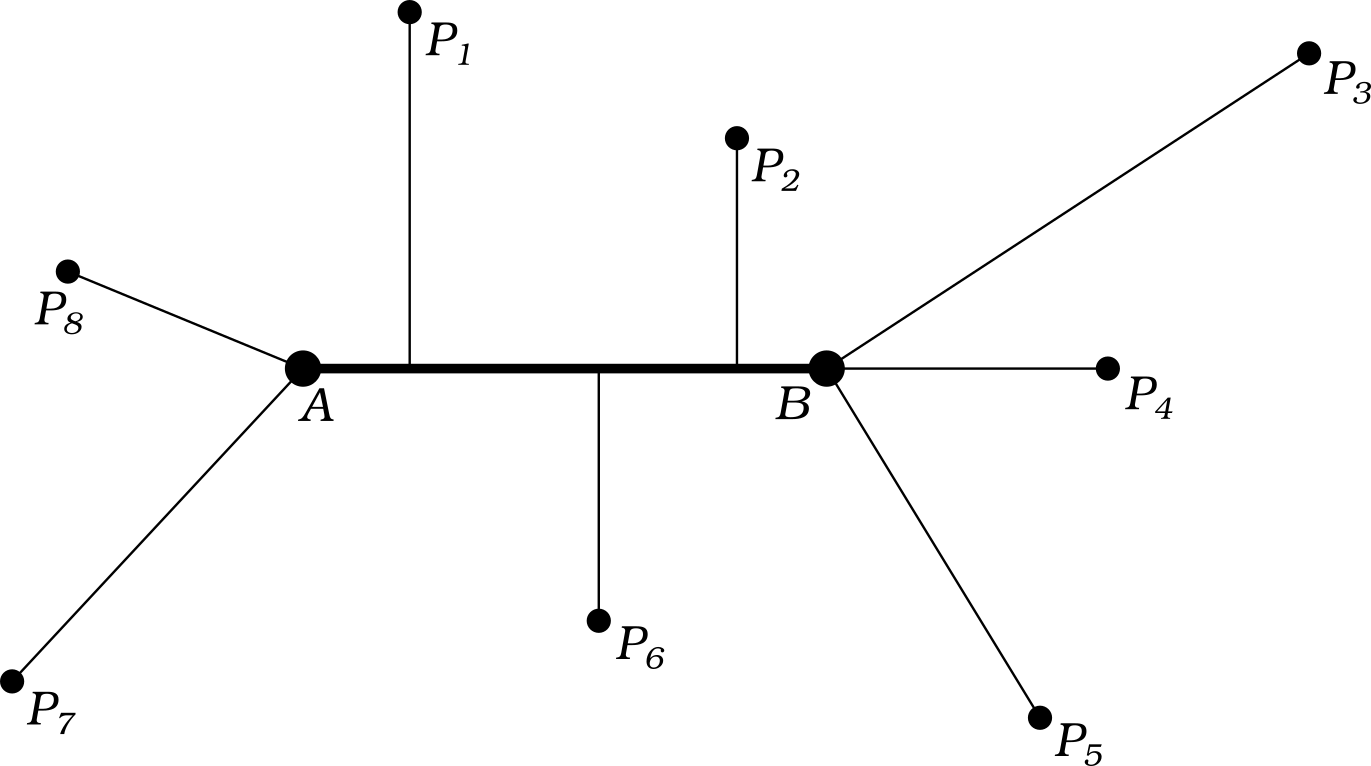
\includegraphics[width=0.6\textwidth]{images/edge_vertex_distance}}
            \caption[Vizualizácia vzdialenosti bodov od hrany]
            {Vizualizácia vzdialenosti bodov $P_1, ..., P_8$ od hrany $E=(A,B)$.}
            %id obrazku, pomocou ktoreho sa budeme na obrazok odvolavat
            \label{obr:edge_vertex_distance}
        \end{figure}

        \begin{figure}
            \centerline{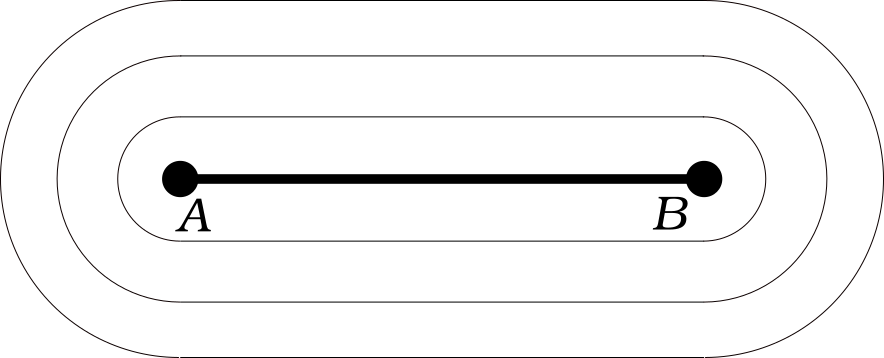
\includegraphics[width=0.4\textwidth]{images/isocurves}}
            \caption[Izočiary metriky]
            {Izočiary metriky z definície \ref{def:segment_point_distance}.}
            %id obrazku, pomocou ktoreho sa budeme na obrazok odvolavat
            \label{obr:isocurves}
        \end{figure}



        Následne sa pokúšame vytvoriť trojuholník spĺňajúci podmienky opísané v kapitole 
        \ref{kap:triangle_conditions} s týmito vrcholmi počnúc od najbližšieho k hrane.
    }
    \item{
        Nájdeme všetky hraničné vrcholy, ktoré sú k bodu $x_{new}$ bližšie ako $0.4 \, a$
        a pokúšame sa vytvoriť trojuholník s týmito bodmi počnúc od najbližšieho k \mbox{hrane $E$}. 
        Tento krok sa nenachádzal v pôvodnom algoritme avšak považujeme ho za dôležitý, 
        keďže ako dôsledok nespájania blízkych bodov môžu neskôr vznikať úzke alebo malé trojuholníky. 
        Príklad využitia tohto kroku môžeme vidieť na \newline\mbox{obrázku \ref{obr:close_points}}. 
        \begin{enumerate}[a)]
            \item{
                Trojuholník $T_{new}$ spĺňa \textit{Delaunayovu podmienku}, teda podľa základného 
                algoritmu pridáme trojuholník do meshu. Zdalo by sa nám však správne vytvoriť a 
                pridať do meshu trojuholník $T_{prev} = (x_i, x_j, x_{prev})$. 
            }
            \item{
                Keďže v okolí bodu $x_{new}$ sa nachádza vrchol $x_{prev}$, pokúsime
                sa vytvoriť trojuholník s bodom $x_{prev}.$
            }
            \item{
                Trojuholník $T_{prev} = (x_i, x_j, x_{prev})$ spĺňa \textit{Delaunayovu podmienku},
                a teda ho pridáme do meshu. 
            }
        \end{enumerate}
        
        \begin{figure}
            \centerline{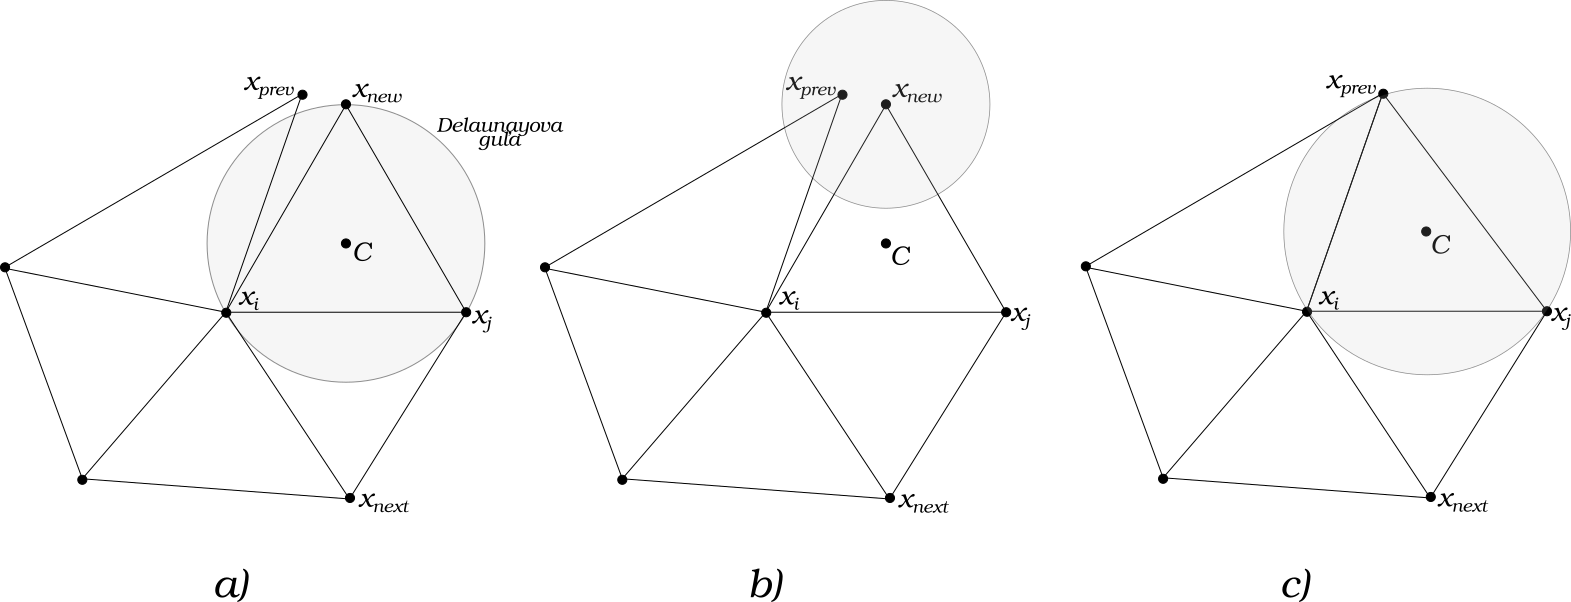
\includegraphics[width=1\textwidth]{images/close_points}}
            \caption[Trojuholník spĺňajúci Delaunayovu podmienku]
            {Trojuholník $T_{new}$ spĺňa Delaunayovu podmienku.}
            %id obrazku, pomocou ktoreho sa budeme na obrazok odvolavat
            \label{obr:close_points}
        \end{figure}
    }
    \item{
        Nájdeme najbližšiu hranu k bodu $x_{new}$, opäť používame metriku z definície 
        \ref{def:segment_point_distance}. Ak je táto hrana bližšie ako $\frac{a}{3}$, 
        pokúsime sa vytvoriť trojuholník s koncovými bodmi hrany, ak ani tieto trojuholníky 
        nie sú vyhovujúce, pokúsime sa vytvoriť trojuholník so stredom najbližšej hrany.
        Tento krok pridávame, pretože
        tieto vrcholy sa nám zdajú ako vhodný kandidáti na vytvorenie nového trojuholníka
        aj napriek tomu, že nemusia byť objavené \textit{Delaunayovou podmienkou} ani ako 
        blízke body k bodu $x_{new}$. V tomto prípade sme uvažovali nad dvoma prístupmi. 
        Prvý je len pripnúť 
        bod na stred hrany, druhý je daný bod najprv premietnuť na povrch a následne k nemu bod 
        pripnúť. V druhom prípade je triangulácia presnejšia avšak v prvom vyzerá na pohľad 
        prirodzenejšie. Postup môžeme vidieť na obrázku \ref{obr:closest_edge} kde
        v časti $d)$ ilustrujeme druhý prístup.

        \begin{figure}
            \centerline{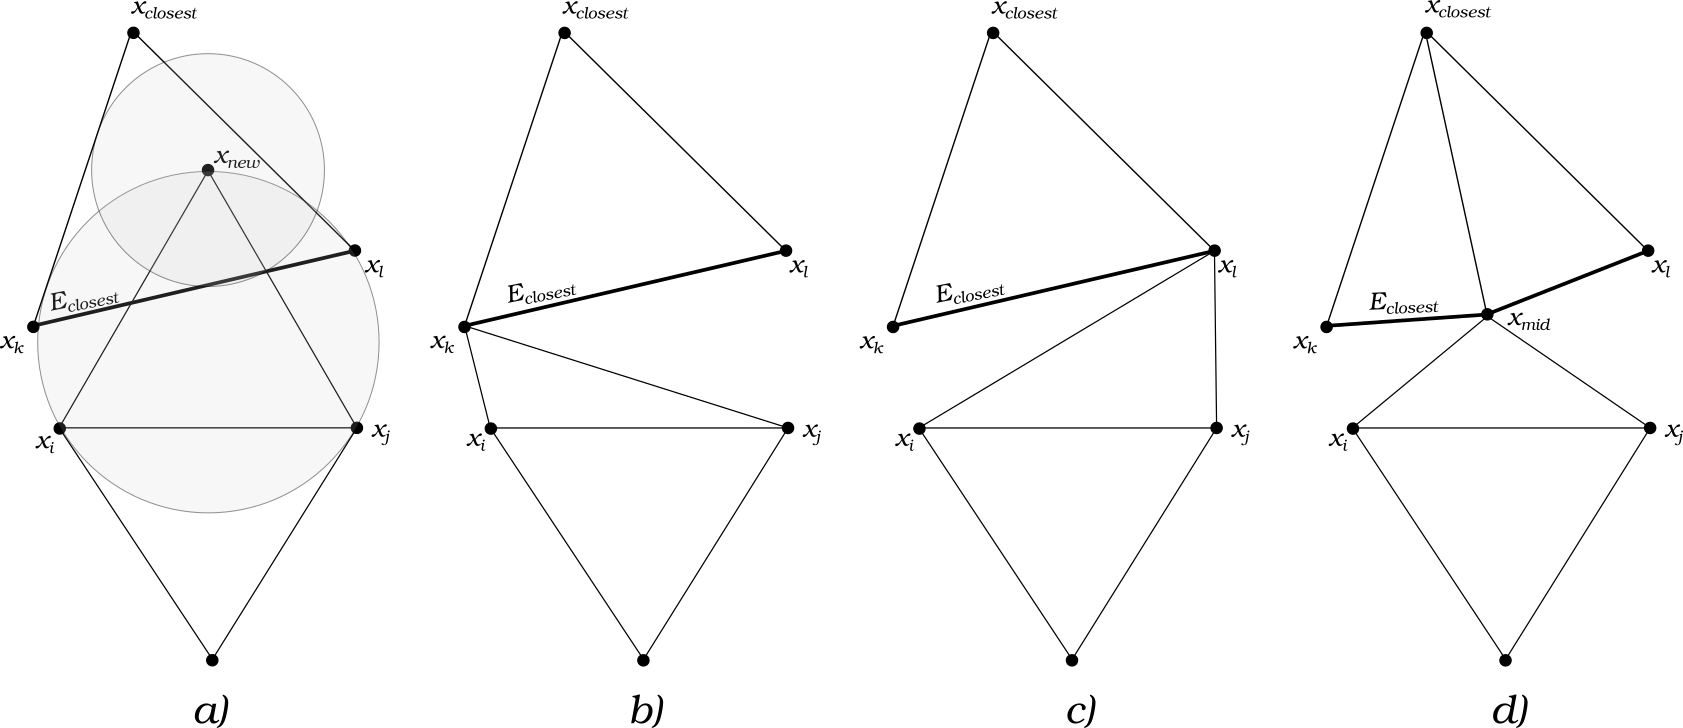
\includegraphics[width=1\textwidth]{images/closest_edge}}
            \caption[Spájanie nového bodu s vrcholmi najbližšej hrany]
            {Spájanie bodu $x_{new}$ s vrcholmi najbližšej hrany $E_{closest}$.}
            %id obrazku, pomocou ktoreho sa budeme na obrazok odvolavat
            \label{obr:closest_edge}
        \end{figure}
    }
    \item{
        Ak sa nám doteraz nepodarilo vytvoriť nový trojuholník a trojuholník $T_{new} = (x_i, x_j, x_{new})$
        spĺňa podmienky z kapitoly \ref{kap:triangle_conditions}, pridáme ho do meshu a skončíme.
    }
    \item{
        Ak sa nám nepodarilo pridať ani trojuholník $T_{new}$, pokúsime sa vytvoriť trojuholníky 
        $T_{prev} = (x_i, x_j, x_{prev})$ a $T_{next} = (x_i, x_j, x_{next})$.
    }
    \item{
        Ak sa nám nepodarilo vytvoriť nový trojuholník, označíme hranu $E = (x_i, x_j)$ za skontrolovanú
        a skončíme.
    }
    Algoritmus beží pokým nie sú všetky zostávajúce hrany v zozname hrán skontrolované. 
    Dôležité je si uvedomiť, že predchádzajúci postup negarantuje topologickú korektnosť
    triangulácie. Prípady topologických nezhôd sú však ojedinelé a súvisia najmä so zvolením príliš
    veľkej dĺžky hrany trojuholníka $a$.

    Po algoritme môžu v meshi takisto zostať diery, ich uzatváranie budeme riešiť v nasledujúcej kapitole.
\end{enumerate}

\section{Uzatváranie dier}
\label{kap:second_part_of_algorithm}
Ako si všimli aj autori článku \cite{akkouche2001adaptive}, po algoritme vznikajú v meshi 
\textit{praskliny} a \textit{diery}. Vďaka našim zmenám v algoritme sa však vo výslednom modeli nachádza minimum dier 
a vďaka Delaunayovej podmienke máme garantované, že šírka diery nepresahuje veľkosť hrany trojuholníka
$a$. Pri vypĺňaní dier teda už iba spájame existujúce vrcholy meshu a nevytvárame žiadne nové.
Na obrázku \ref{obr:models_after_first_part} môžeme vidieť výsledky algoritmu opísaného v 
predchádzajúcej podkapitole. Pre horšiu viditeľnosť sú zostávajúce diery zakrúžkované.

\begin{figure}
    \centerline{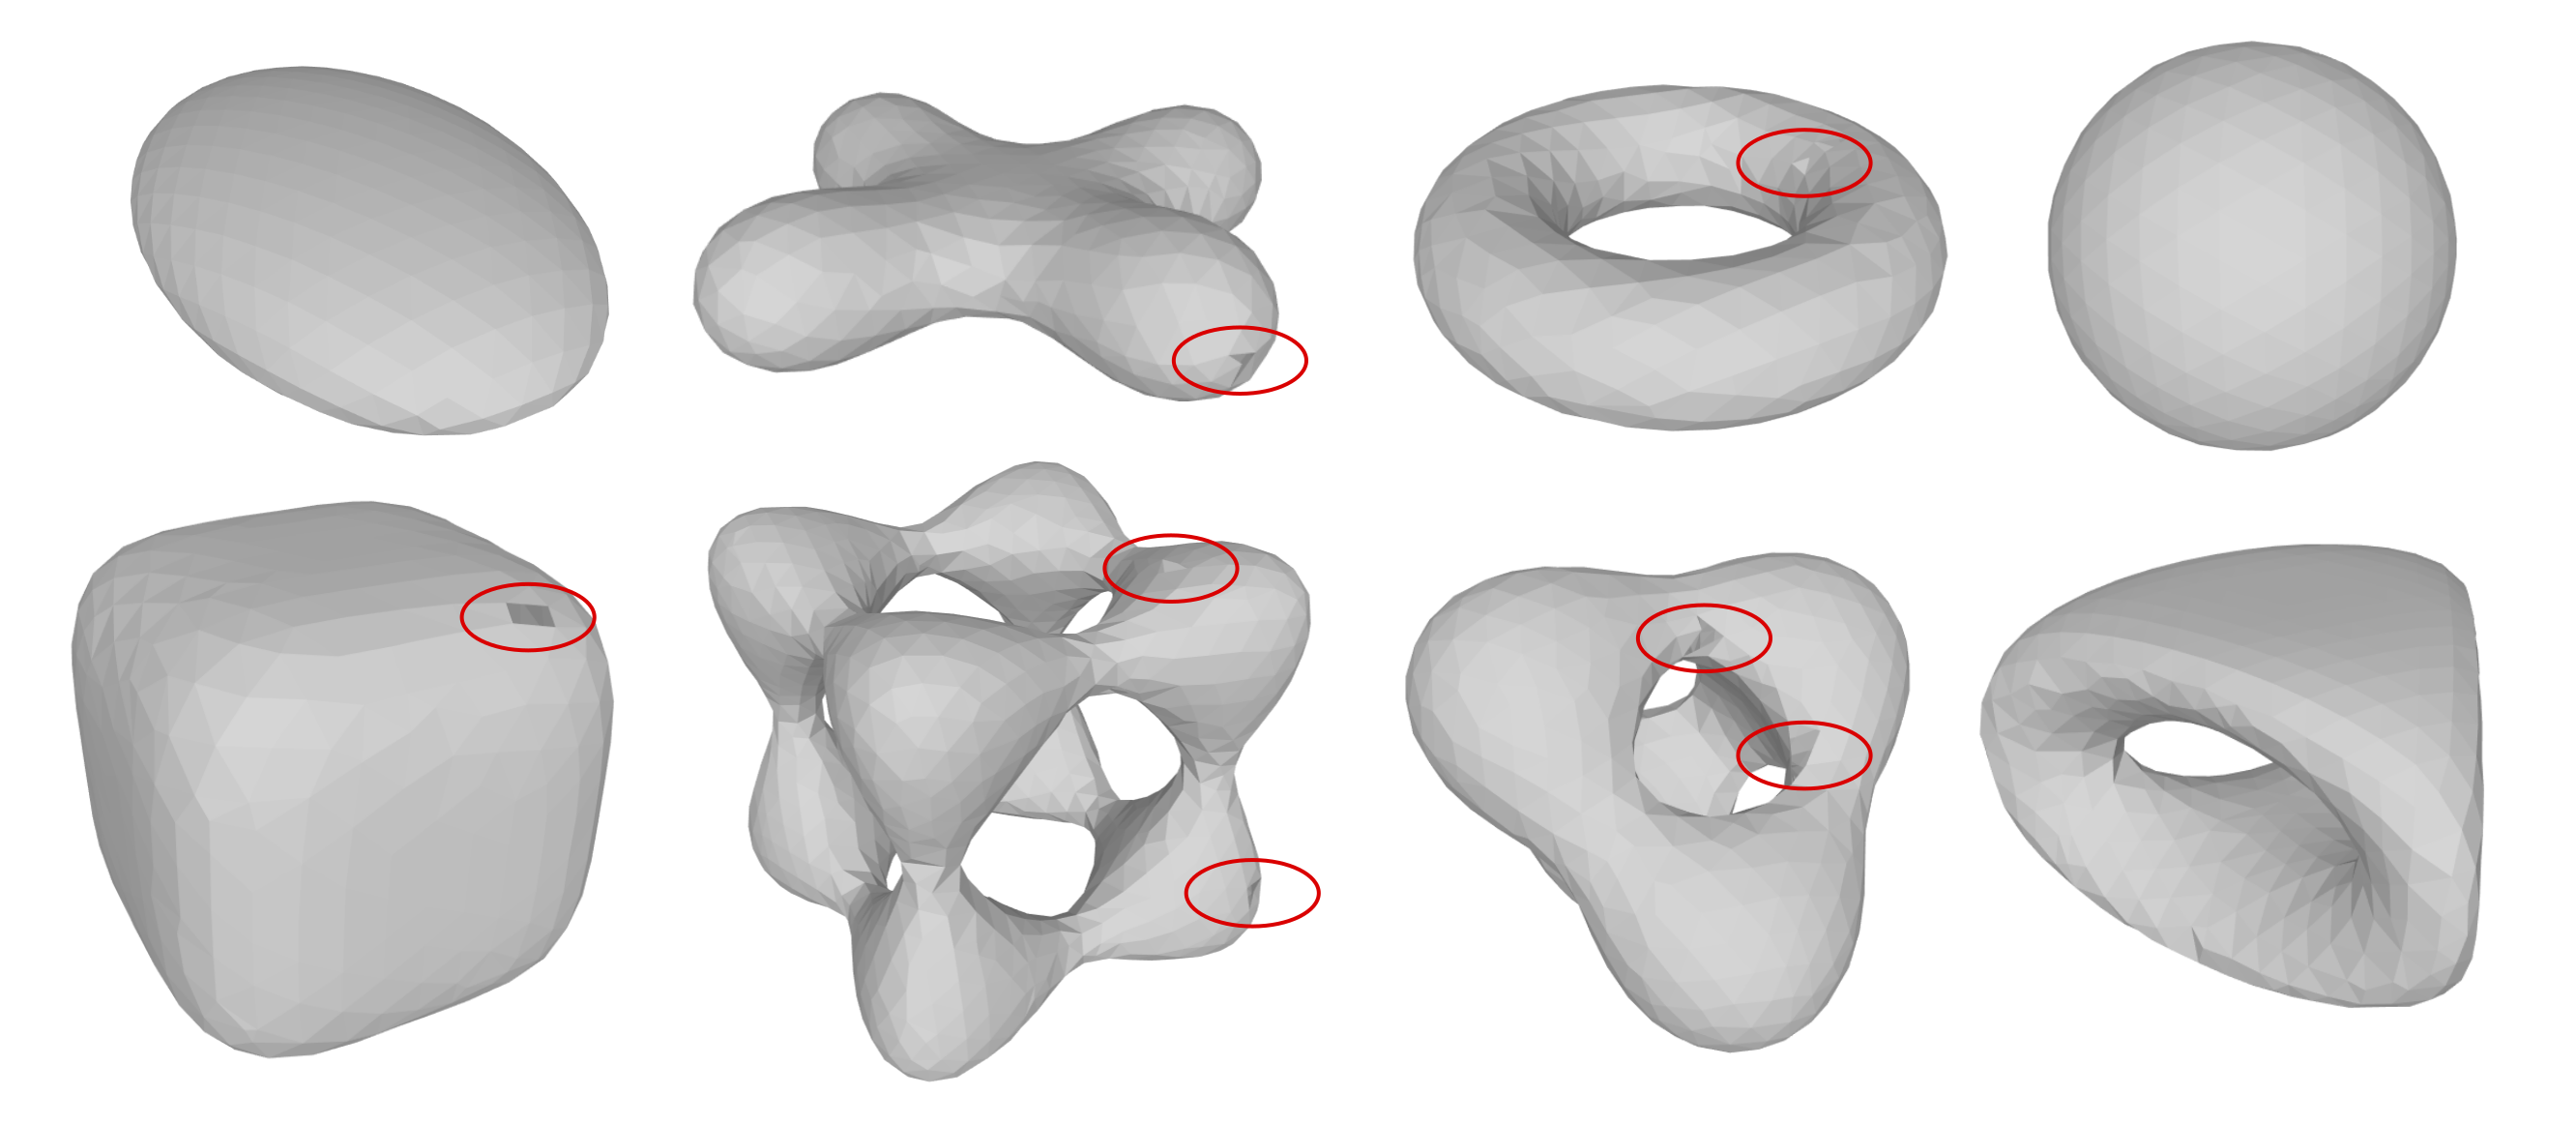
\includegraphics[width=1\textwidth]{images/models_after_first_part}}
    \caption[Diery v modeloch]
    {Diery v modeloch zostávajúce po prvej časti algoritmu.}
    %id obrazku, pomocou ktoreho sa budeme na obrazok odvolavat
    \label{obr:models_after_first_part}
\end{figure}

\subsection{Algoritmus pre uzatváranie dier}

Po skončení prvého algoritmu nemáme žiadne neskontrolované hrany. Avšak v prípade, že v meshi zostali 
diery, zostávajú v zozname skontrolované hrany, kú ktorým sme nenašli trojuholník. V nasledujúcom 
algoritme vynechávame \textit{Delaunayovu podmienku} a takisto podmienku overujúcu blízkosť ťažiska. 
Dôvod nutnosti vynechania tejto podmienky pri uzatváraní dier sme opísali v bode 4. v kapitole 
\ref{kap:triangle_conditions}.

Skontrolované hrany si pred spustením algoritmu označíme opäť za neskontrolované. V každom kroku vyberieme
zo zoznamu jednu hranu a vykonáme nasledujúce kroky.
\begin{enumerate}
    \item{
        V prípade, že $x_{prev} = x_{next}$, teda v meshi je diera v tvare trojuholníka, pridáme tento 
        trojuholník do meshu. Tento krok vykonávame aj v prvej časti algoritmu. Väčšina zostávajúcich
        dier je práve v tvare trojuholníka, preto je tento krok vhodný, nekomplikovaný a rýchly.
    }
    \item{
        Nájdeme najbližší vrchol $x_{closest}$ k hrane $E = (x_i, x_j)$, ktorý spĺňa všetky podmienky 
        opísané v kapitole \ref{kap:triangle_conditions} okrem Delaunayovej podmienky a podmienky 
        kontrolujúcej ťažisko trojuholníka a zároveň je k hrane $E$ bližšie ako $1.5 \, a$. 
        Opäť používame metriku 
        opísanú v definícii \ref{def:segment_point_distance}. Ak sa takýto vrchol podarí nájsť, 
        vytvoríme trojuholník $T_{closest} = (x_i, x_j, x_{closest})$ a pridáme ho do meshu.
    }
    \item{
        Ak sa nám nepodarilo vytvoriť trojuholník s najbližším vrcholom, opäť sa pokúšame vytvoriť 
        trojuholníky s vrcholmi porušujúcimi \textit{Delaunayovu podmienku} počnúc od najbližšieho, 
        potom s vrcholom $x_{prev}$
        a nakoniec s vrcholom $x_{next}$. Všetky bez overovania \textit{Delaunayovej podmienky} a 
        podmienky s ťažiskom.
    }
    \item{
        Ak sa nám aj tak nepodarilo vytvoriť nový trojuholník, označíme hranu za skontrolovanú a prejdeme
        na ďalšiu.
    }
    
    Ak po skončení aj druhej časti algoritmu zostávajú nevyriešené hrany, nepodarilo sa nám 
    uzatvoriť všetky diery. Tento prípad však nenastáva príliš často. Ak nastane, tak zväčša pri 
    príliš veľkých trojuholníkoch kvôli ktorým sa v prvej časti algoritmu vytvorili topologicky
    nekonzistentné trojuholníky. Ako však poznamenali aj S. Akkouche a E. Galin 
    \cite{akkouche2001adaptive}, je bežné vymeniť garanciu topologickej korektnosti za rýchlosť,
    či výslednú kvalitu meshu. 
\end{enumerate}

\section{Ohraničená triangulácia}
\label{kap:bounded_triangulation}
Keďže algoritmus je implementovaný ako prechod cez zoznam všetkých hrán okraja a tento zoznam 
sa priebežne mení, skončenie algoritmu máme garantované iba pri ohraničených plochách.
Ak chceme triangulovať aj neohraničené plochy, je nutné pridať \textit{ohraničujúcu obálku}, 
ktorú sme spomenuli aj v kapitole \ref{kap:input_data}.

\subsection{Nutné kroky pri tvorbe ohraničenej triangulácie}

V tejto podkapitole popíšeme nad akými krokmi sa potrebujeme zamýšľať, ak chceme vytvoriť prirodzene 
vyzerajúcu ohraničenú plochu. Presné prevedenie
ako docieliť takúto ohraničenú trianguláciu na vstupnom trojrozmernom intervale 
$I = \langle x_{min}, x_{max} \rangle \times \langle y_{min}, y_{max} \rangle \times 
\langle z_{min}, z_{max} \rangle$ opíšeme v kapitole \ref{kap:implementation}.

\begin{itemize}
    \item{
        Pri tvorbe nového vrchola kontrolujeme, či sa nachádza vnútri ohraničujúcej obálky.
    }
    \item{
        Nové vrcholy nachádzajúce sa vonku z ohraničenej obálky vhodne premietame na obálku.

        Ak by sme tento krok vynechali, ohraničenie by síce fungovalo a algoritmus by v nejakom
        momente skončil, avšak ohraničenie by nebolo presné a vyzeralo by neprirodzene.
    }
    \item{
        Vrcholy, ktoré sú vnútri avšak blízko obálky pripíname na obálku.

        Pri vynechaní tohto kroku vznikajú pri okraji veľmi úzke a malé trojuholníky, čomu 
        sa v ideálnom prípade chceme vyhnúť.
    }
    \item{
        Hľadáme rozumné riešenie pripínania vrcholov na hrany a rohy obálky, aby boli hrany 
        \textit{ostré} 
        a nie \textit{odseknuté}. Na obrázku \ref{obr:cut_corners} môžeme vidieť, čo myslíme pod 
        \textit{ostrými} rohmi. Vidíme trianguláciu časti plášťa valca, pri ktorej sme zámerne pre
        lepšiu názornosť zvolili
        pomerne veľkú veľkosť hrany trojuholníka, vľavo má tento valec 
        \textit{odseknuté} rohy a napravo ich má \textit{ostré}. My sa budeme snažiť o dosiahnutie
        \textit{ostrých} rohov.

        \begin{figure}
            \centerline{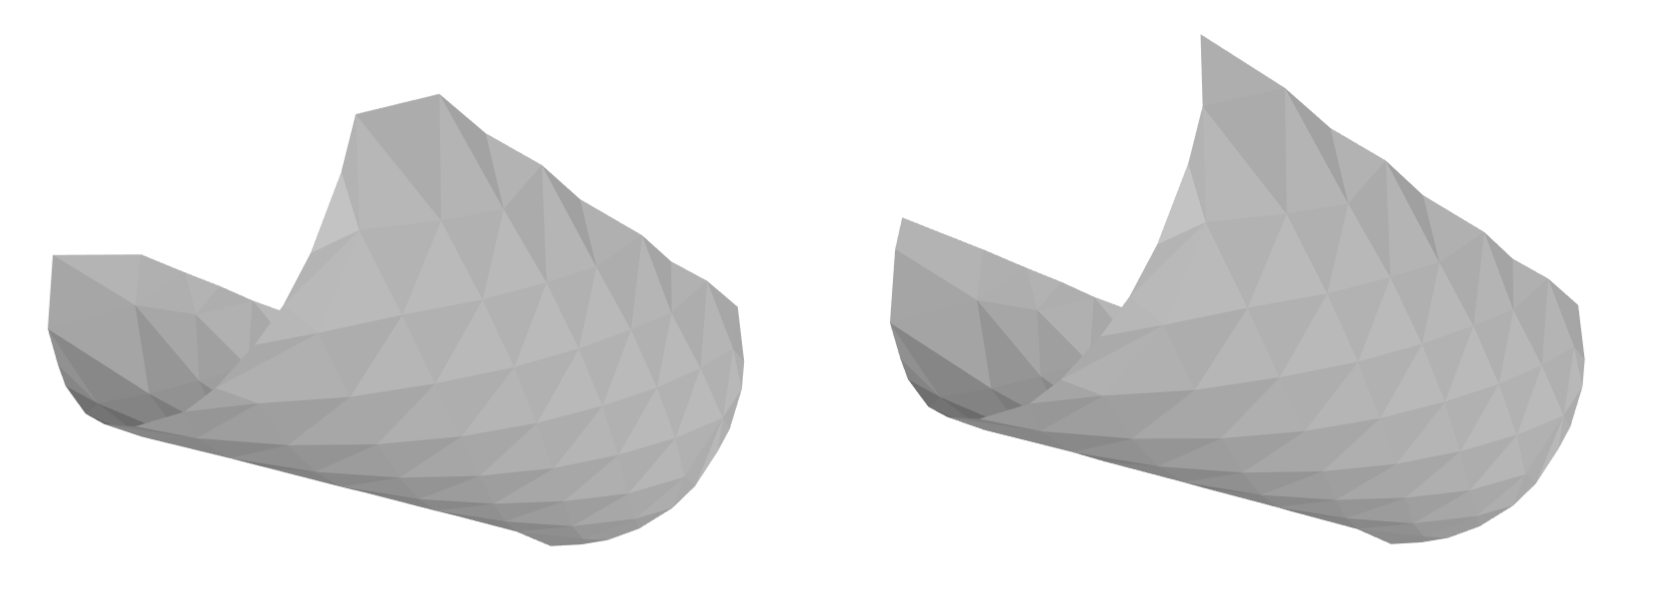
\includegraphics[width=1\textwidth]{images/cut_corners}}
            \caption[\textit{Ostré} a \textit{odseknuté} rohy pri ohraničenej triangulácii]
            {\textit{Odseknuté} rohy pri ohraničenej triangulácii (vľavo), \textit{ostré} rohy (vpravo).}
            %id obrazku, pomocou ktoreho sa budeme na obrazok odvolavat
            \label{obr:cut_corners}
        \end{figure}
    }
\end{itemize}

\subsection{Pripínanie vrcholov na ohraničujúcu obálku}

Spomínali sme, že sme uvažovali o dvoch spôsoboch.
Prvý spôsob, nad ktorým sme uvažovali bolo premietanie blízkych bodov vnútri obálky aj 
bodov vonku z obálky na najbližší bod na obálke. Teda premietanie v smere normál stien obálky.
Tento prístup sme otestovali a ukázalo sa, že má vážny nedostatok a to ten, že premietnuté 
vrcholy boli často príliš ďaleko od plochy a vytvárali nepresný a zúbkovaný okraj plochy. 
Z tohto dôvodu
sme zvolili iný prístup, pri ktorom takisto nie je garantovaná poloha bodu na ploche, avšak 
chyba je oveľa menšia. Tento prístup je premietanie bodu $x_{new}$ na steny obálky v smere 
ťažnice trojuholníka $T = (x_i, x_j, x_{new})$ vedúcej cez bod $x_{new}$.

Na obrázku \ref{obr:crop_to_box} môžeme vidieť oba prístupy. Premietanie v smere normály 
na obrázkoch $a)$ a $b)$, premietanie v smere ťažnice na obrázkoch $c)$ a $d)$. Na prvý pohľad 
výsledky nevyzerajú veľmi rozdielne, avšak v kapitole \ref{kap:results} uvidíme pozitívny vplyv 
na výslednú trianguláciu. 
        
\begin{figure}
    \centerline{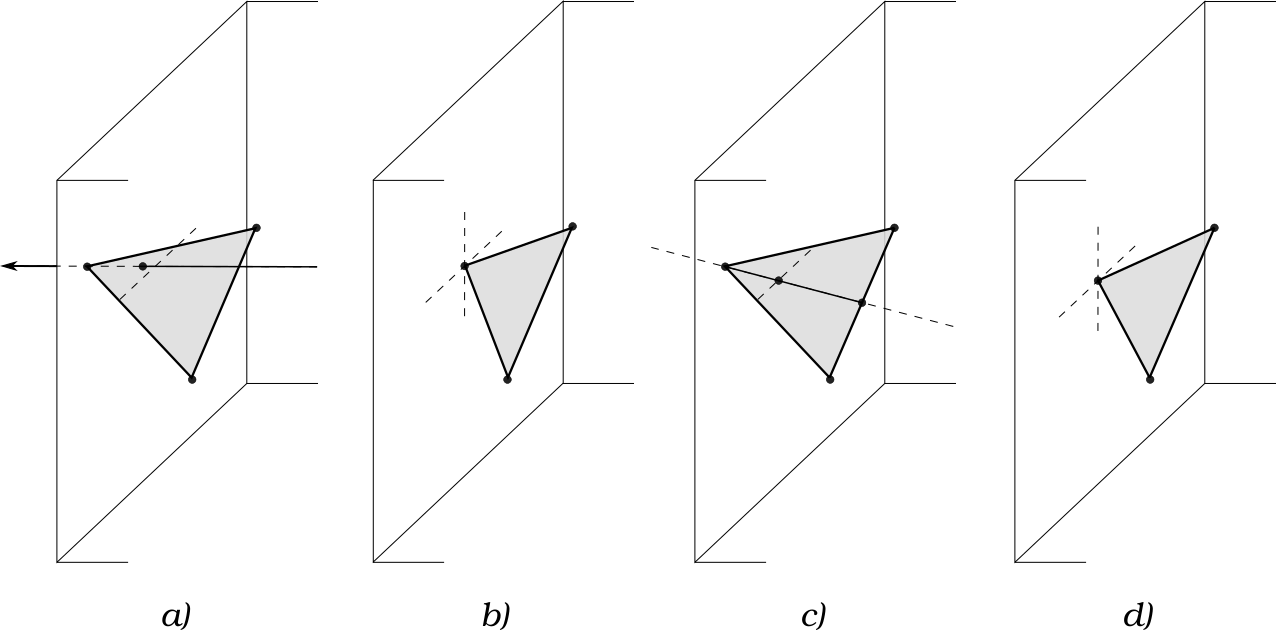
\includegraphics[width=1\textwidth]{images/crop_to_box}}
    \caption[Orezávanie na ohraničujúcu obálku]
    {Prichytávanie na najbližší bod(vľavo), premietanie na obálku v smere ťažnice(vpravo)}
    %id obrazku, pomocou ktoreho sa budeme na obrazok odvolavat
    \label{obr:crop_to_box}
\end{figure}

\subsection{Pripínanie vrcholov na hrany a rohy obálky}

Nazvime ohraničujúce hrany také, ktorých oba konce ležia na ohraničujúcej obálke.
                
Na začiatku nájdeme medzi ohraničujúcimi hranami tie, ktorých konce neležia
na tej istej stene ohraničujúcej obálky. 
Nazvime takúto hranu $E_{ij} = (x_i, x_j)$. Vytvoríme nový trojuholník 
$T_{rim} = (x_i, x_j, x_{rim})$. 

Nazvime $p_{rim}$ priamku prechádzaujúcu 
hranou ohraničujúcej obálky, ktorú majú spoločnú steny, na ktorých ležia 
vrcholy $x_i$ a $x_j$. Vrchol $x_{rim}$ nájdeme ako priesečník priamky $p_{rim}$ 
so zadanou implicitne definovanou plochou, ktorý je najbližší k hrane $E_{ij}$. 
Ak tento priesečník neleží na hrane ohraničujúcej obálky, nastavíme vrchol $x_{rim}$ 
ako najbližší roh ohraničujúcej obálky k tomuto priesečníku.

V prípade, že niektorý z bodov $x_i, x_j$ leží na hrane obálky, nastavíme vrchol
$x_{rim}$ ako roh ohraničujúcej obálky.
Opísaný postup môžeme vidieť na obrázku \ref{obr:fix_corners}. Červenou farbou je vyznačená 
hrana ležiaca na dvoch rôznych stenách, krížikom nový bod a zelenou
farbou nový trojuholník.

\begin{figure}
    \centerline{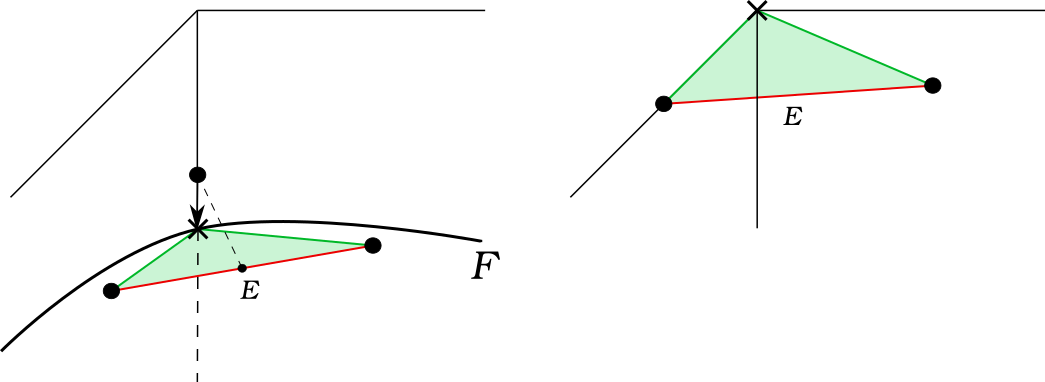
\includegraphics[width=0.7\textwidth]{images/fix_corners}}
    \caption[Prichytávanie na hrany a rohy ohraničujúcej obálky]
    {Prichytávanie na hrany a rohy ohraničujúcej obálky.}
    %id obrazku, pomocou ktoreho sa budeme na obrazok odvolavat
    \label{obr:fix_corners}
\end{figure}

\section{Adaptívna triangulácia}

Algoritmus vytvárajúci adaptívnu trianguláciu povrchu je taký, ktorý vytvára menšie trojuholníky v oblasti 
s väčším zakrivením a naopak v oblastiach s menším zakrivením vytvára väčšie trojuholníky.
Prvý spôsob ako môžeme dosiahnuť takéto správanie je zvoliť vzdialenosť $k$ pri tvorbe vrchola $x_{proj}$
ako výšku rovnostranného trojuholníka so stranou veľkosti $\|e\| = | x_i \, x_j |$, teda 
$k=\frac{\sqrt 3}{2} \| e \|$ avšak stáva sa, že susedné
hrany majú úplne rozdielnu dĺžku, čo môže spôsobiť nepríjemnosti pri spájaní týchto hrán. 
Preto je dobrý nápad zvoliť vzdialenosť $k$ ako výšku rovnostranného trojuholníka so stranou veľkosti
$\| \overline{e} \| = \frac{| x_{prev} \, x_i | + | x_i \, x_j | + | x_j \, x_{next} |}{3}$, čo je 
priemer dĺžok hrany
$E = (x_i, x_j)$ a jej susedných hrán, teda volíme $k=\frac{\sqrt 3}{2} \| \overline{e} \|$. 
Ako uviedli autori S. Akkouche a E. Galin \cite{akkouche2001adaptive}
hlavným nedostatkom tohto prístupu je, že po tom ako vytriangulujeme oblasť s vysokým zakrivením 
veľkosť trojuholníkov zostane malá aj v rovnejších oblastiach. Takisto predstavili riešenie tohto 
problému definovaním minimálnej vzdialenosti $k_{min}$. Následne, ak je $k < k_{min}$ 
nastavíme k na hodnotu $k = \frac{3}{4} \, k + \frac{1}{4} k_{min}$. Takto zaručíme, že $k$ nikdy neklesne
pod hodnotu $\frac{1}{4} k_{min}$. 
Vo všetkých adaptívnych prípadoch sa ešte poisťujeme maximálnou výškou trojuholníka, a to tak, že
výška nemôže presiahnuť $2$--násobok zadanej dĺžky hrany $a$.

V algoritme sa takisto môže stať, že v smere $\nabla F(x_{proj})$ numerické metódy nenájdu koreň. 
Vo všeobecnosti koreň v tomto smere ani nemusí existovať. Takéto správanie takisto naznačuje, že oblasť
môže mať veľké zakrivenie. Navrhujeme teda v prípade neúspešnosti premietania na plochu v smere gradientu 
zmenšiť veľkosť $k$ na $0.8 k$, pričom pri opätovnom neúspechu tento proces môžeme opakovať aj viac 
krát. 

Ďalší fakt naznačujúci veľké zakrivenie povrchu je skalárny súčin normál trojuholníka $N$ pri hrane $E$
a nového trojuholníka $T_{new}$ menší ako nejaká hodnota $\alpha_{min}$, v tomto prípade tiež navrhujeme
zmenšiť veľkosť $k$ na $0.8 k$ a premietať znova, pričom pri opätovnom neúspechu tento proces 
môžeme opakovať aj viac krát.

Posledný prístup, ktorý v našej práci predstavíme patrí medzi najjednoduchšie a to prerozdeľovanie 
trojuholníkov už existujúcej triangulácie. Naše kritérium na rozhodnutie prerozdelenia trojuholníka
je vzdialenosť ťažiska $t$ trojuholníka od bodu $t_{proj}$, ktorý nájdeme premietnutím $t$ na plochu
v smere $\nabla F(t)$. Ak je táto vzdialenosť väčšia ako $d_{max}$, potom trojuholník prerozdelíme 
na menšie trojuholníky. Jednoduchý avšak nie ideálny prístup je rozdeliť trojuholník na 3 nové 
trojuholníky tak ako vidíme na obrázku \ref{obr:triangle_splitting} vľavo. 

\begin{figure}
    \centerline{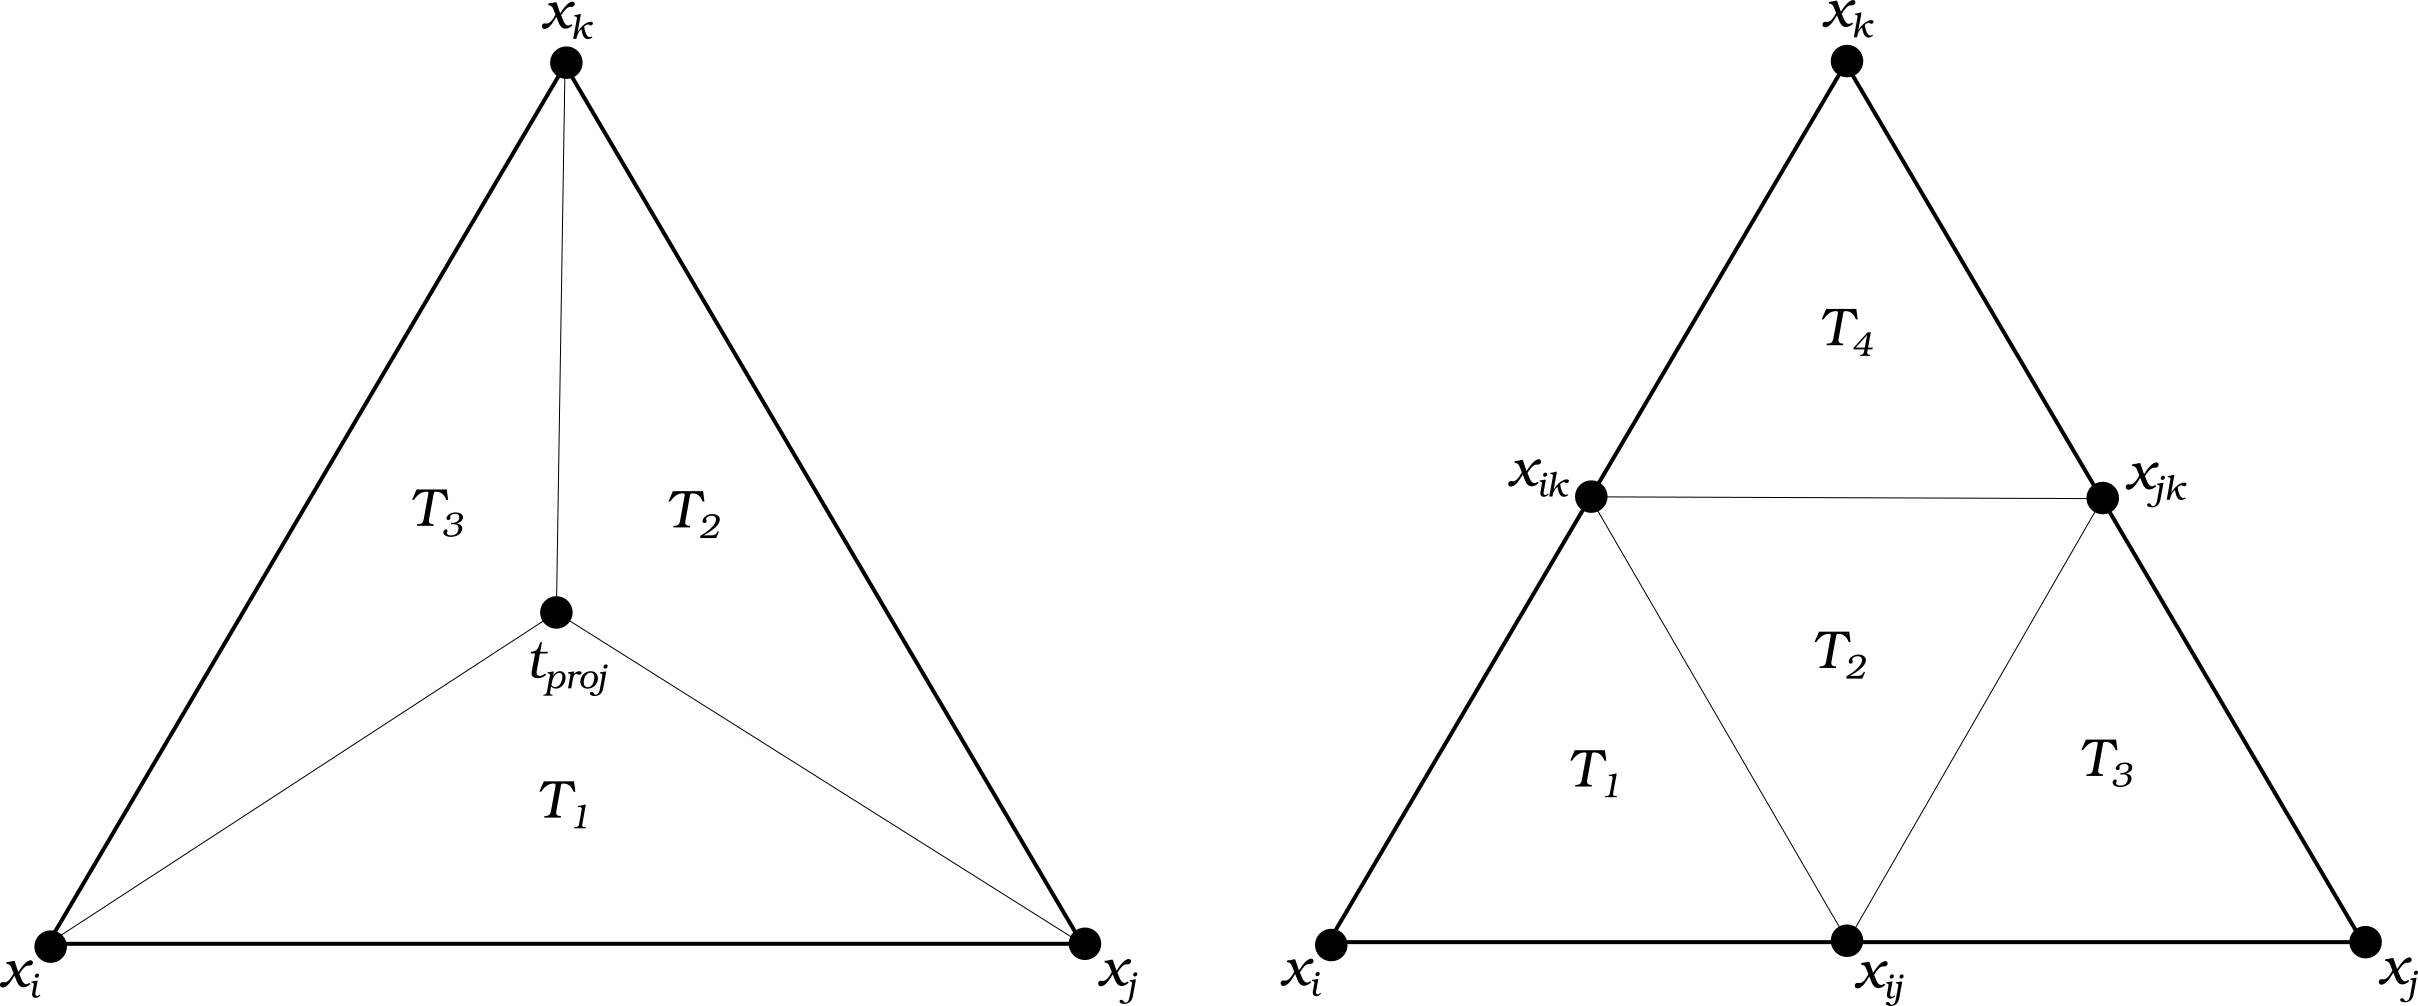
\includegraphics[width=0.7\textwidth]{images/triangle_splitting}}
    \caption[Spôsoby adaptívneho podrozdelenia trojuholníka]
    {Spôsoby adaptívneho podrozdelenia trojuholníka.}
    %id obrazku, pomocou ktoreho sa budeme na obrazok odvolavat
    \label{obr:triangle_splitting}
\end{figure}

Spôsob prerozdelenia 
trojuholníka na 4 nové trojuholníky ilustrovaný vpravo vyzerá omnoho lepšie, nové vrcholy
volíme ako stredy strán trojuholníka. Pri tomto postupe je však potrebné riešiť vznikajúce diery.
Tieto diery vznikajú medzi dvoma trojuholníkmi ak jeden z nich prerozdeľujeme
a druhý nie. Na obrázku \ref{obr:holes_while_splitting} vľavo vidíme vzniknutú dieru po premietnutí bodu
$x_{jk}$ na plochu. Napravo vidíme naše riešenie. Ak susedný trojuholník taktiež prerozdeľujeme, nový bod
premietneme na plochu, inak ho ponecháme ako stred hrany. Na obrázku \ref{obr:holes_while_splitting} vpravo
vidíme trojuholník $T=(x_i, x_j, x_k)$, ktorý chceme prerozdeliť. Pozrieme sa na jeho susedné trojuholníky.

Trojuholník $N_{ij}$, ktorý je susedný k hrane $E_{ij} = (x_i, x_j)$ neprerozdeľujeme, preto vrchol $x_{ij}$ 
nepremietame na plochu a nechávame ho uprostred hrany $E_{ij}$. Takisto ani trojuholník $N_{ik}$ neprerozdeľujeme,
a tak aj vrchol $x_{ik}$ zostáva nepremietnutý na plochu.
Trojuholník $N_{jk}$ však prerozdeľujeme a tak, vrchol $x_{jk}$ premietame na plochu. To či na plochu premietneme aj 
zvyšné dva stredy strán trojuholníka $N_{jk}$ závisí zase od jeho susedných trojuholníkov. 
V tejto ilustácii ich však premietame na povrch, preto sú hrany trojuholníka $N_{jk}$ lomené.

Tento prístup je implementovaný ako 
prechod cez všetky trojuholníky meshu. Ak je ťažisko ďaleko, teda chceme trojuholník prerozdeliť
pozrieme sa na susedné trojuholníky. Podľa nich rozhodneme, ktoré zo stredov strán premietneme,
a ktoré ponecháme nepremietnuté.

\begin{figure}
    \centerline{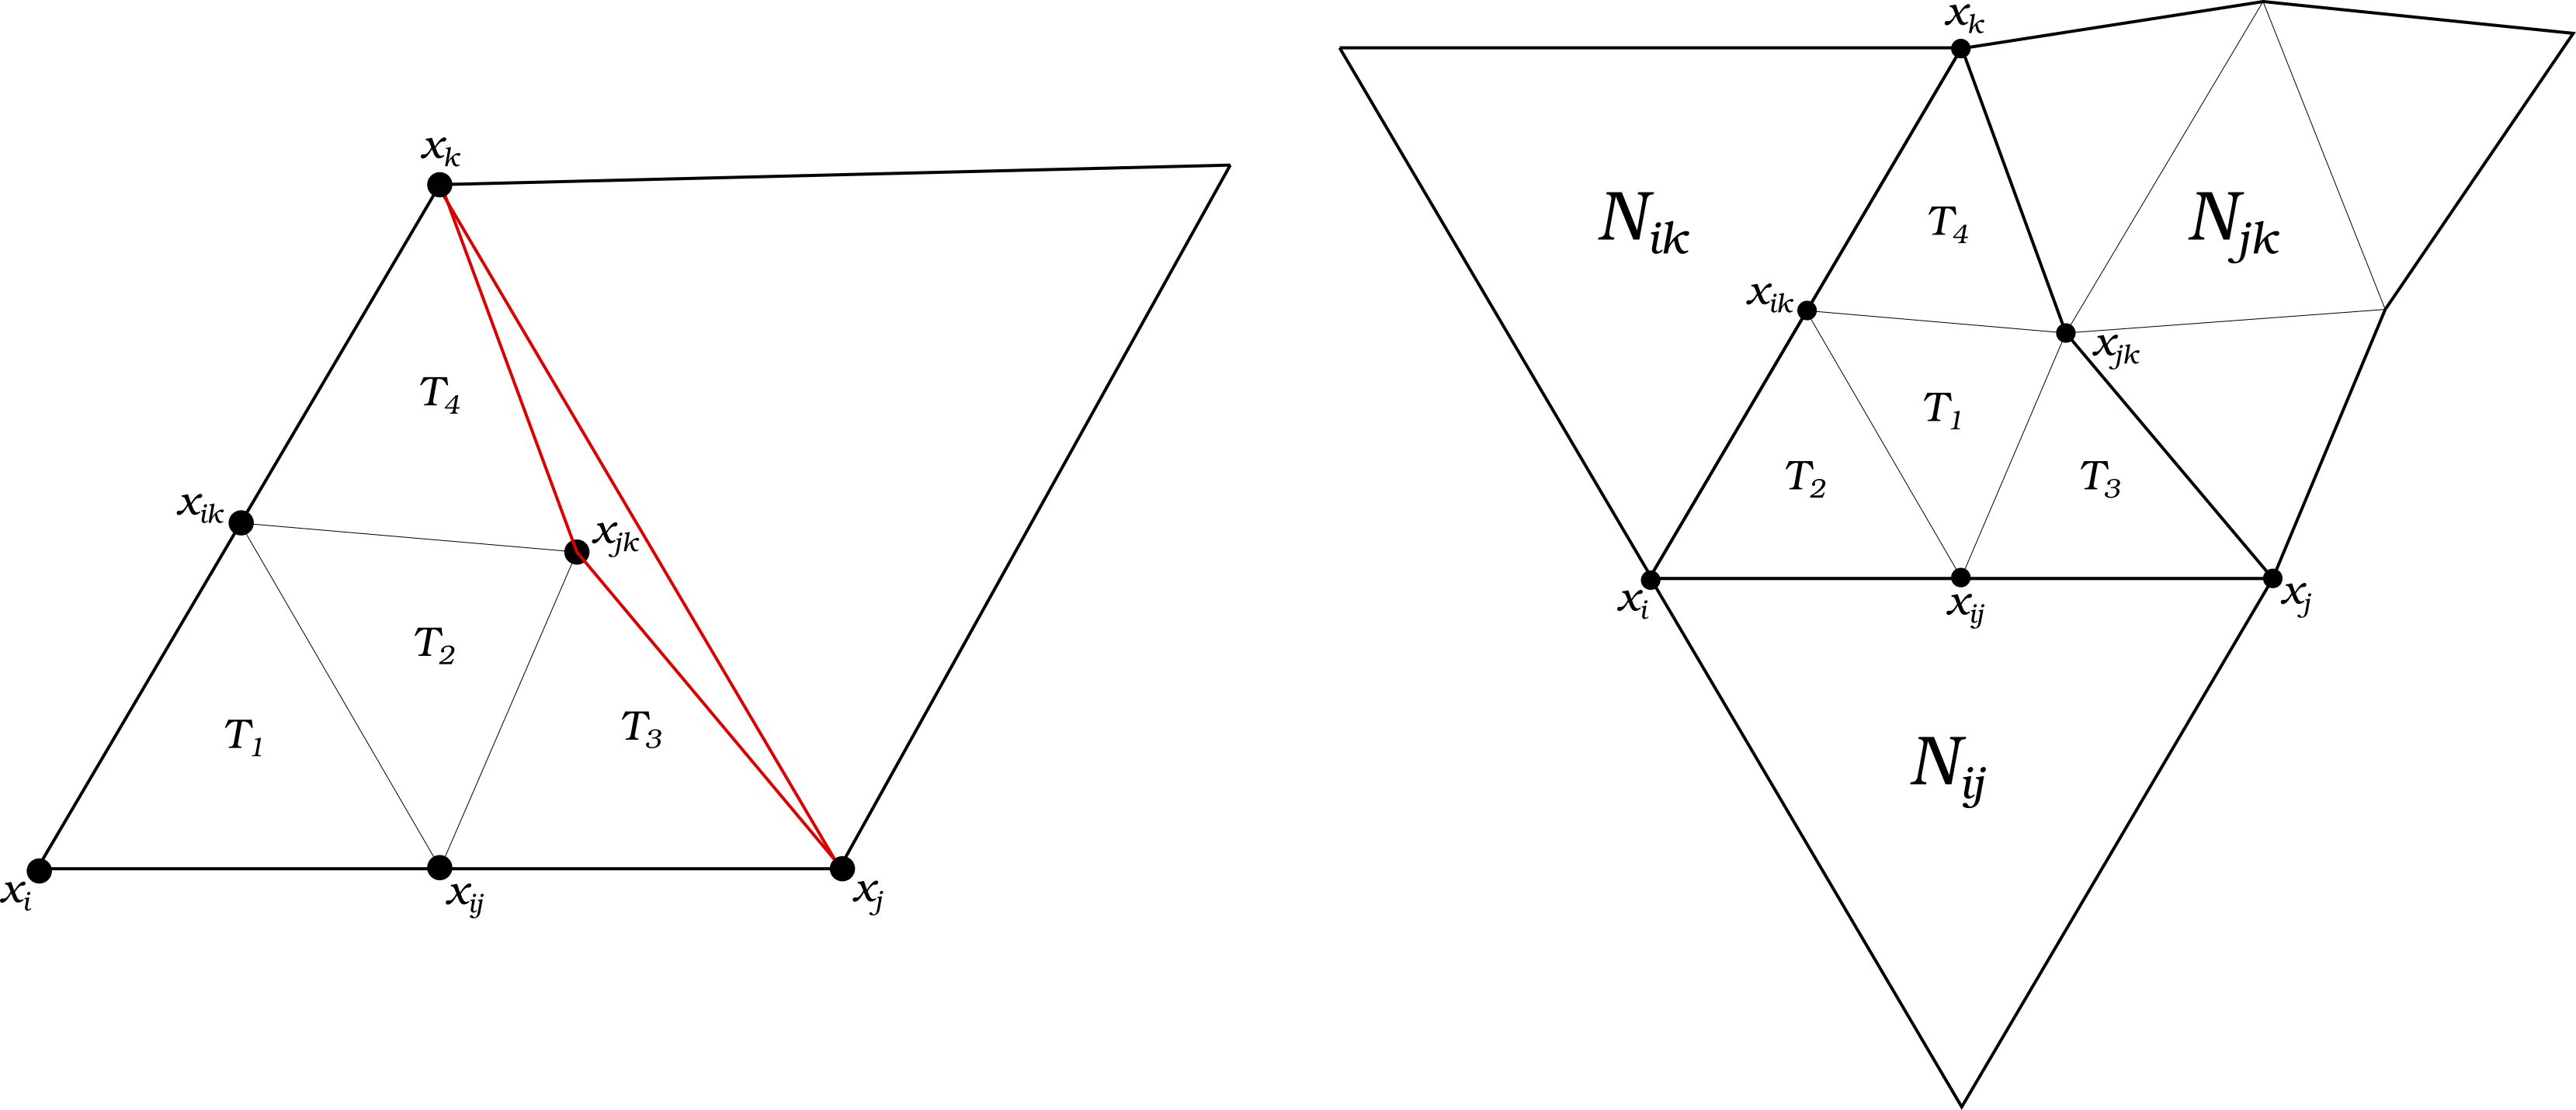
\includegraphics[width=1\textwidth]{images/holes_while_splitting}}
    \caption[Úprava adaptívneho podrozdelenia trojuholníkov]
    {Diera vzniknutá pri adaptívnom prerozdelení iba niektorých trojuholníkov(vľavo), 
    navrhované riešenie(vpravo).}
    %id obrazku, pomocou ktoreho sa budeme na obrazok odvolavat
    \label{obr:holes_while_splitting}
\end{figure}